\documentclass[twoside,leqno, 11pt]{article}

\usepackage[svgnames, table]{xcolor}
\usepackage{cmap}
\usepackage{graphicx} 
\usepackage{wrapfig}
\usepackage{lastpage}
\usepackage{tikz}
\usepackage{multirow}
\usetikzlibrary{calc}
\usepackage{pgfplots}
\pgfplotsset{width=7cm,compat=1.8}
\usepackage{braket}
\usepackage{verbatim}
\usetikzlibrary{arrows}
\usetikzlibrary{calc,positioning,fit,backgrounds}
\usetikzlibrary{decorations.pathreplacing,calc}
\usepackage{amsmath} 
\allowdisplaybreaks
\usepackage[T2A]{fontenc}
\usepackage[utf8]{inputenc}	
\usepackage[english,russian]{babel}
\usepackage{geometry}
\geometry{top=16mm}
\geometry{bottom=16mm}
\geometry{left=16mm}
\geometry{right=16mm}	
\usepackage{amssymb}
\usepackage{listings}
\lstset{language=R,
    basicstyle=\small\ttfamily,
    stringstyle=\color{DarkGreen},
    numberstyle=\tiny\color{DarkRed}, 
    rulecolor=\color{black},
    morekeywords={TRUE,FALSE},
    deletekeywords={data,frame,length,as,character},
    keywordstyle=\color{DarkBlue},
    commentstyle=\color{DarkGreen},
}       
\usepackage{icomma} 
\usepackage{mathtext} 
\usepackage{mathrsfs}
\usepackage{mathtools}
\usepackage{fancyhdr}
\pagestyle{fancy}
\fancyhf{}
\renewcommand{\headrulewidth}{0,04mm}
\usepackage{hyperref}
\usepackage{mathtext} 
\usepackage{multicol}
\chead{\scshape{Tutorial on Active Inference \\ Весна 2020}}
%\lhead{}
%\chead{\date{\today}} 
\cfoot{\thepage} 
%\hypersetup{
%  colorlinks=true
%   linkcolor=red,       
%        citecolor=black,   
%        filecolor=magenta, 
%        urlcolor=blue}
\makeatletter % сделать "@" "буквой", а не "спецсимволом" - можно использовать "служебные" команды, содержащие @ в названии
\renewcommand{\headrulewidth}{0,6mm} 

\renewcommand{\maketitle}{\begin{center}
	\noindent{\bfseries\scshape\LARGE\@title}\par
\noindent {\large\scshape\bfseries\@subtitle}\par
\noindent {\large\slshape\mdseries\@author}
\vskip 2ex
\end{center}}

\DeclareMathOperator*{\plim}{plim}
\DeclareMathOperator{\var}{Var}
\newcommand{\lag}{\mathcal{L}}
\newcommand{\e}{\mathbb{E}}
\newcommand{\p}{\mathbb{P}}
\newcommand{\n}{\mathcal{N}}


\pgfmathdeclarefunction{gauss}{2}{%
        \pgfmathparse{1/(#2*sqrt(2*pi))*exp(-((x-#1)^2)/(2*#2^2))}%
    }

\renewcommand{\maketitle}{\noindent{\bfseries\scshape\LARGE\@title}\par
        
\noindent {\slshape\mdseries\@author}
\vskip 2ex}

\renewcommand\section{\@startsection{section}{1}{\z@}%
        {-3.5ex \@plus -1ex \@minus -.2ex}%
        {-1em}%
        {\normalfont\large\scshape\bfseries}}

%\renewcommand\subsection{\@startsection{subsection}{1}{\z@}%{-3.5ex \@plus -1ex \@minus -.2ex}%       {-1em}%{\normalfont\bfseries}}
\renewcommand*\env@matrix[1][*\c@MaxMatrixCols c]{%
  \hskip -\arraycolsep
  \let\@ifnextchar\new@ifnextchar
  \array{#1}}
  \newenvironment{sqcases}{%
  \matrix@check\sqcases\env@sqcases
}{%
  \endarray\right.%
}
\def\env@sqcases{%
  \let\@ifnextchar\new@ifnextchar
  \left\lbrack
  \def\arraystretch{1.2}%
  \array{@{}l@{\quad}l@{}}%
}
\makeatother

%\title{Problem Set 2}
\author{Махнева Елизавета, Брсикян Бабкен \\ БЭК171}

\begin{document}
	
\section*{Предисловие от авторов}~\

	Данная статья является переводом \href{https://medium.com/@solopchuk/tutorial-on-active-inference-30edcf50f5dc}{Tutorial on Active Inference} Олега Солопчука. Так как тема Свободной Энергии является достаточно новой в научной среде, в этой статье присутствует много терминов, которые не очень популярны, с которыми русский читатель встречается впервые. В связи с чем очень тяжело перевести их на русский язык точно, потому что в русском языке такие словосочетания и слова не имеют определенного смысла. Но мы постарались перевести все максимально корректно и, более того, решили оставить некоторые термины в квадратных скобках на оригинальном(английском) языке для того, чтобы предоставить читателям возможность перевести самим, если их не устроит текущий перевод.

\section*{Статья}~\

	Активный вывод[Active inference] -- это принцип Свободной Энергии[Free Energy principle] мозга, применяемый к действию. Этот принцип относительно подтверждается экспериментами в области нейронаук и является популярной моделью работы мозга. В нашей статье, мы рассмотрим последнюю версию, которая сформулирована как planning in discrete state-space and time. Изначальная предпосылка автивного вывода[initial inference]: агент(любая самоорганизующаяся система) хочет остаться в живых, поддерживая свой гомеостаз. В конце концов, агент должен обеспечить себя соблюдением того, чтобы важные для существования параметры(температура тела или оксигенация крови) не отклонялись сильно от нормы, т.е. чтобы не были неожиданными[surprising]. Но поскольку эти параметры можно вывести только с помощью сенсорных измерений, агент минимизирует неожиданность[surprise] наблюдений, полученных с помощью сенсоров. Интересно то, что данная задача схожа с задачей продолжительного улучшения модели мира, воспринимаемой агентом(убедимся в этом позже). Рассмотрим вышеописанную схему вкратце:
	
\begin{center}
	Остаться в живых $\Rightarrow$ подерживать гомеостазис $\Rightarrow$ избегать неожиданных[surprisng] состояний $\Rightarrow$ избегать неожиданных[surprisng] наблюдений $\Rightarrow$ минимизация приближения к неожиданностям[свободной энергии]
\end{center}
	
	И если \href{https://medium.com/@solopchuk/intuitions-on-predictive-coding-and-the-free-energy-principle-3fc5bcedc754}{предыдущий пост} нацелен был на то, чтобы дать интуицию Свободной энергии[Free Energy], то здесь нам придется испачкать ручки. Никакого технического бэкграунда не нужно, за исключением \href{https://www.mathsisfun.com/data/probability.html}{Теории вероятностей} и \href{https://www.mathsisfun.com/data/bayes-theorem.html}{Теоремы Байеса}

	\textbf{Мозг избегает неожиданностей[surprise], имея хорошую модель окружающей среды}. С одной стороны, окружение имеет истинную, скрытую для агента, случайную величину \textbf{s} (называемую состояние), которая генерирует вероятностные наблюдения [probabilistic observations] \textbf{o}. Важно подчеркнуть, что состояние \textbf{s} скрытое означает, что мы можем наблюдать только \textbf{o}. Например, шел дождь ночью (\textbf{s}), значит трава влажная утром (\textbf{o}). Это называется генеративным процессом [Generative process] $R(s,o)$.
	
	%\vspace{-3mm}
	\begin{figure}[h]
		\centering{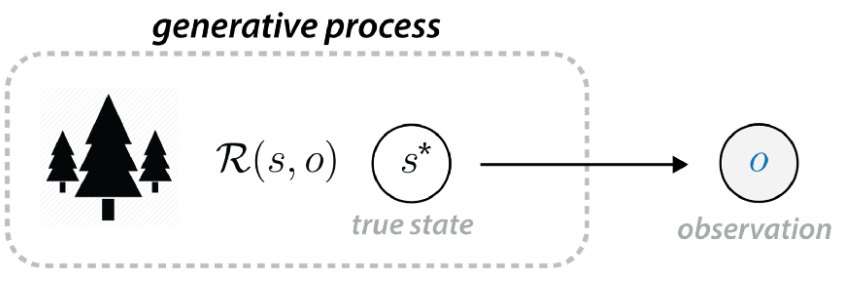
\includegraphics[width=0.45\linewidth]{one}}
		\label{ris:image}
	\end{figure}
	%\vspace{-3mm}
	
	С другой стороны, мозг пытается сделать заключение[infer] о вероятности разных скрытых состояний[states], учитывая наблюдения, $p(s|o)$. И делает он это через приорные знания[prior belief] $p(s)$ и правдободобие[likelihood] $p(o|s)$. Таким образом, мозг строит генерируемый процесс[generative process] определяемую as a joint $p(s,o)$.

	%\vspace{-3mm}
	\begin{figure}[h]
		\centering{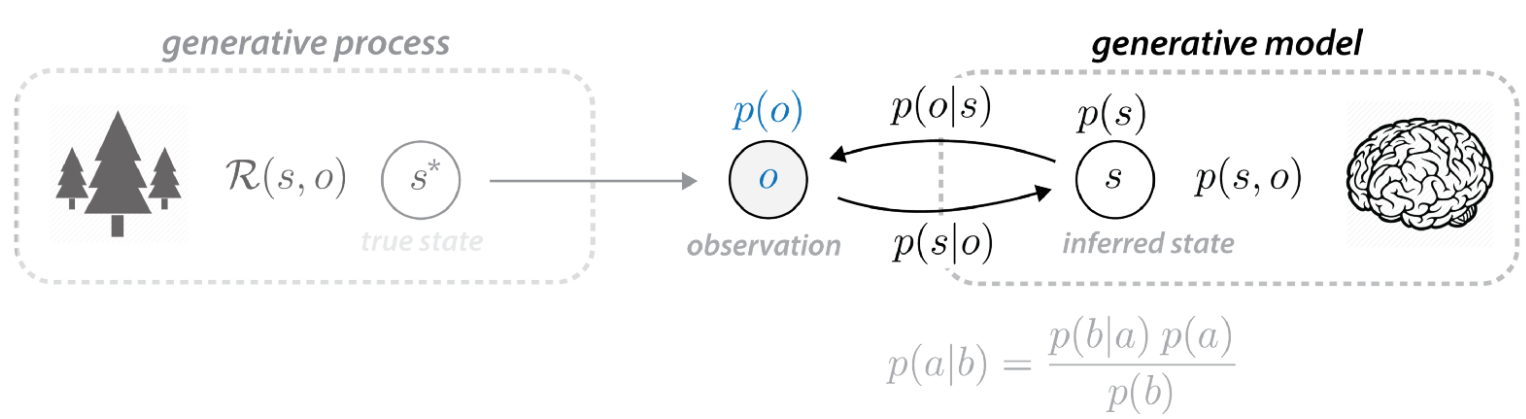
\includegraphics[width=0.75\linewidth]{two}}
		\label{ris:image}
	\end{figure}
	%\vspace{-3mm}
	
	Давайте рассмотрим пример. Представим следующий генеративный процесс[generative proces] - в нашем саду яблочное и апельсиновое дерево. Обозначим за скрытую переменную \textbf{s} - является фрукт апельсином или яблоком. Предположим, что яблочное дерево немного левее апельсинового дерева. Итак, когда фрукты падают на землю, мы наблюдаем следующее:

	%\vspace{-3mm}
	\begin{figure}[h]
		\centering{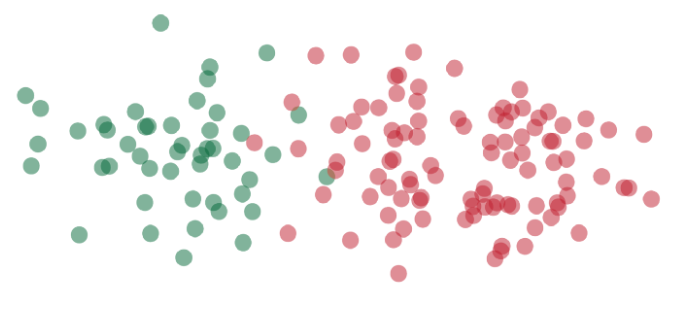
\includegraphics[width=0.5\linewidth]{three}}
		\label{ris:image}
	\end{figure}
	%\vspace{-5mm}
	
	Кажется, что 70\% лежащих фруктов -- апельсины, а остальные 30\% - яблоки. Это истинное распределение скрытого состояния[hidden state] \textbf{s}. Когда фрукты падают, они не попадают в одно и тоже местоположение, они рандомно распространяются вокруг. Это уже вероятность наблюдении при условии \textbf{s}. \textbf{Вывод}[\textbf{Inference}] в генеративной модели[generative model] заключается в нахождении апостериорного распределения $p(s|o)$ -- вероятность того, что фрукт является яблоком, учитывая его местоположения. \textbf{Обучение} генерируемой модели[generative model] состоит из оценивания параметров распределения (таких как, например, математическое ожидание и дисперсия для нормального распределения) скрытого состояния $p(s)$, of the state-observation mapping $p(o|s)$. Вывод $p(s|o)$ через теорему Байеса требует от нас подсчета вероятности $p(o)$, которая интересна собою, учитывая тот факт, что чем лучше наша модель, тем выше будет вероятность наблюдаемых данных $p(o)$. Это также называется 1) 'обоснованность модели'['model evidence'], так как это учитывает как хорошо наша модель предсказывает настоящие данные[real data], 2) 'предельная вероятность'['marginal likelihood'],  потому что мы marginalize, или суммируем скрытое состояние[hidden state] s.
	Сравним 2 модели внизу, которые оценивают $p(o,s)$: модель слева, очевидно, лучше -- $p(s)$ корректно показывает, что апельсинов больше, чем яблок, и $p(o|s)$ хорошо центрирован по всем кластерам. Мы можем количественно оценить качество каждой модели с помощью свидетельства модели $p(o)$, изолируя скрытую переменную s.
	
	%\vspace{-4mm}
	\begin{figure}[h]
		\centering{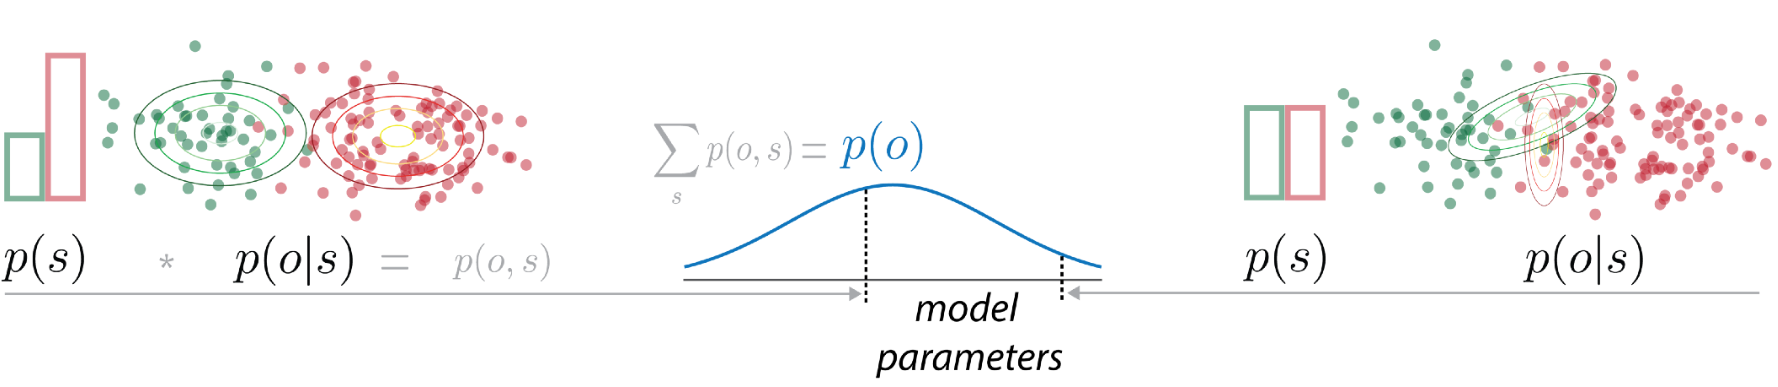
\includegraphics[width=0.9\linewidth]{four}}
		\label{ris:image}
	\end{figure}
	%\vspace{-3mm}
	
	В идеале, мы хотим выбрать такие параметры модели, которые будут вести к насколько возможно лучшему model evidence $p(o)$. Как это связано с активным выводом[active inference] и с агентом, который избегает неожиданных наблюдений? По факту, задача \textbf{максимизации model evidence эквивалентна минимизации неожиданности}, которая всего лишь отрицательный логарифм $p(o)$. Если вероятность равна 1 - неожиданность[surprise] равна 0, вероятность равна 0 - неожиданность[surprise] стремится к бесконечности. Здесь неожиданность[surprise] представлена, как функция от вероятности:
	
	%\vspace{-3mm}
	\begin{figure}[h]
		\centering{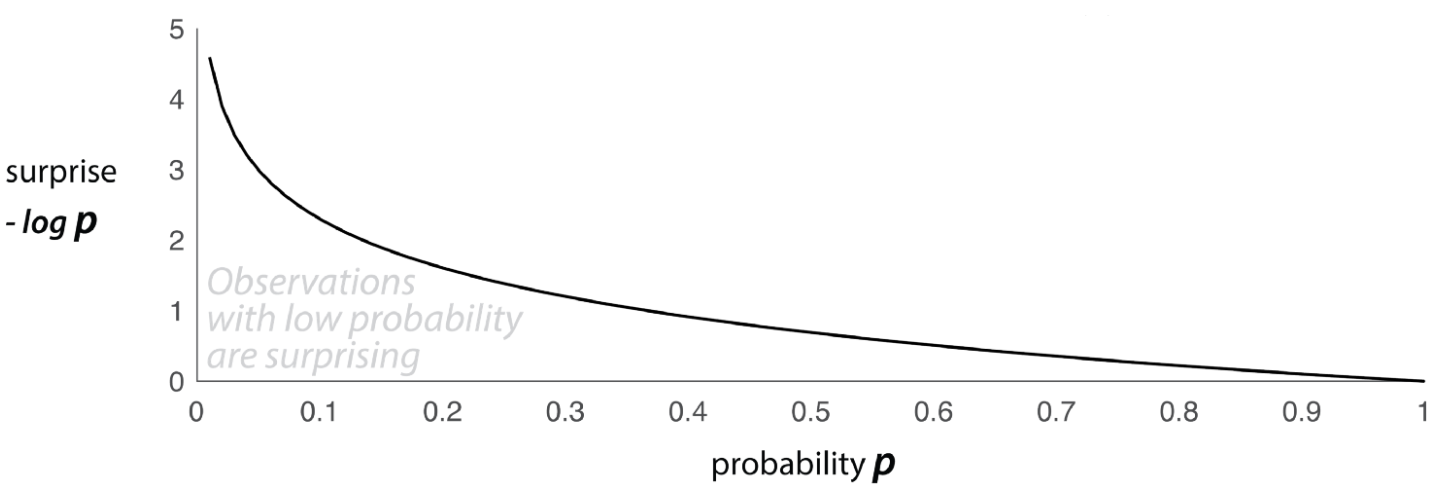
\includegraphics[width=0.7\linewidth]{five}}
		\label{ris:image}
	\end{figure}
	%\vspace{-3mm}
	
	Здесь неожиданность[surprise] $-log$ $p(o)$, overlaid с model evidence $p(o)$:
	
	%\vspace{-3mm}
	\begin{figure}[h!]
		\centering{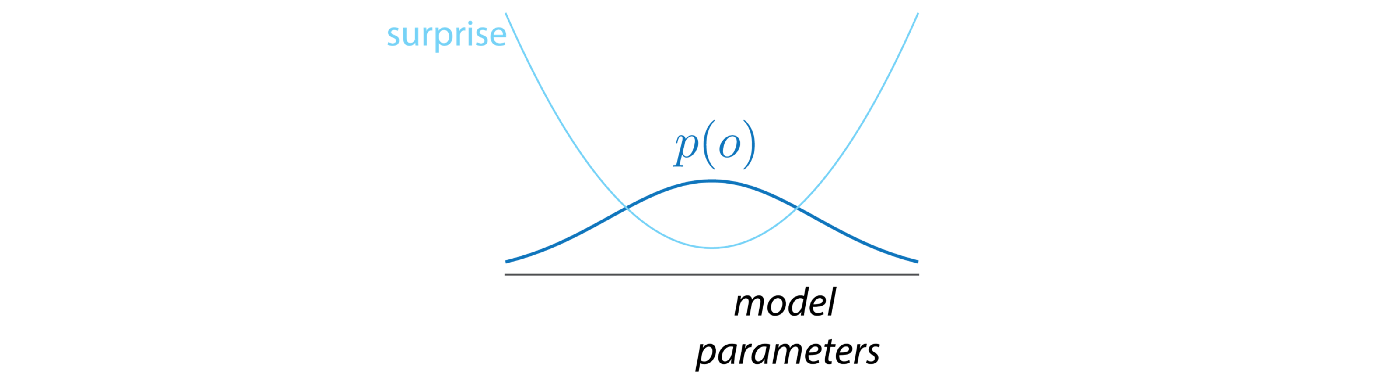
\includegraphics[width=0.3\linewidth]{six}}
		\label{ris:image}
	\end{figure}
	%\vspace{-5mm}
	
	Как мы обсуждали выше для обоснованности модели[model evidence], чтобы оценить неожиданность[surprise] $-log$ $p(o)$, нам  нужно просуммировать по скрытой переменной \textbf{s} совместное распределение $p(o, \textbf{s})$:
	
	%\vspace{-3mm}
	\begin{figure}[h!]
		\centering{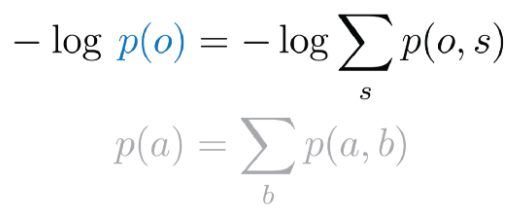
\includegraphics[width=0.3\linewidth]{seven}}
		\label{ris:image}
	\end{figure}
	%\vspace{-4mm}
	
	Так как речь идет о суммировании по всем возможным значениям \textbf{s}, суммирование может стать очень тяжелым занятием, если будет очень много различных значений \textbf{s}. Однако есть трюк, который поможет вам избежать невозможного суммирования.
	
	Вместо того, чтобы считать неожиданность[surprise] прямо, мы можем аппроксимировать ее чем-то очень схожим и легко обрабатываемым. Сперва, мы представляем простое распределение[dummy distribution] q с областью значений s (которая окажется безумно полезной позже). Мы можем спокойно внести ее в сумму через деление и умножение одновременно: 
	
	%\vspace{-4mm}
	\begin{figure}[h!]
		\centering{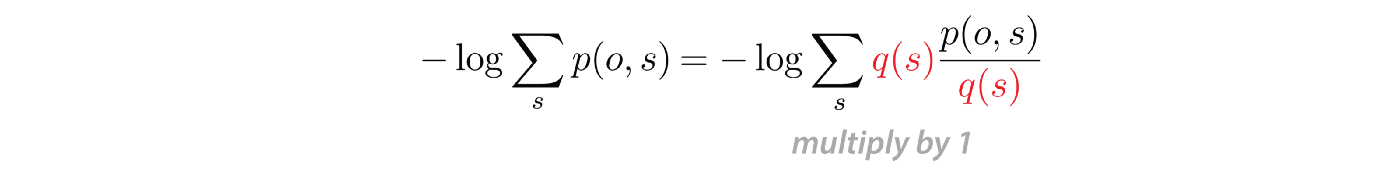
\includegraphics[width=0.4\linewidth]{eight}}
		\label{ris:image}
	\end{figure}
	%\vspace{-4mm}
	
	Это дает нам взвешенную сумму, в которой для каждой s, отношение $p(o, s)/q(s)$ суммируется с весом $q(s)$. Это все еще та же неожиданность[surprise] $-log$ $p(o)$, но теперь нам очень удобно заменить ее аппроксимацией.
	
	Теперь же, давайте отвлечемся от неожиданности[surprise] на секунду и сфокусируемся на аппроксимировании. Мы знаем, что функция неожиданности[surprise] $-log$ выглядит как впадина или чаша(иными словами выпуклая). Определение гласит: функция выпуклая в том случае, если когда вы уроните на нее палку, палочка окажется в функции, как в миске. Формально мы объясняем это следующим образом. Давайте возьмем 2 точки на оси абсцисс (\textbf{x} и \textbf{y}), и выберем число между 0 и 1 (\textbf{w}). Как показано ниже, мы можем двигаться между \textbf{x} и \textbf{y} с помощью их взвешенной суммы через изменение \textbf{w} от 0 до 1. То есть мы могли бы рассматривать \textbf{w} и (1 - \textbf{w}) как параметры обычного распределения[simple distribution]. На самом деле, есть краткое название для «взвешенных сумм, в которых веса определяются распределением» -- \href{https://en.wikipedia.org/wiki/Expected_value}{математическое ожидание}. Теперь вернемся к тетиве в луке: если вы оцениваете функцию этого ожидания, она всегда будет ниже или равна ожиданию функции, оцененной в \textbf{x} и \textbf{y}.
	
	%\vspace{-4mm}
	\begin{figure}[h]
		\centering{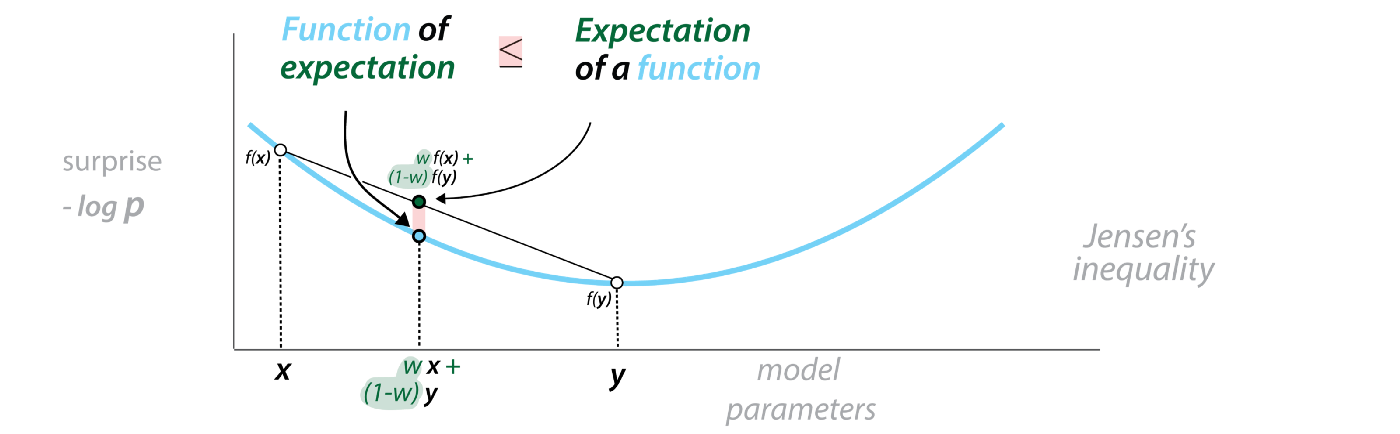
\includegraphics[width=0.65\linewidth]{nine}}
		\label{ris:image}
	\end{figure}
	%\vspace{-3mm}
	
	Поскольку ранее мы обозначили неожиданность[surprise], как функцию (-log) от математического ожидания (взвешенной суммы отношения $p(o, s) / q(s)$), то неравенство выпуклости[inequality of convexity] выглядит подходящей для нашего приближения! Формально, это называется «верхняя граница». И вот, эта верхняя граница... Свободная энергия.
	
	%\vspace{-3mm}
	\begin{figure}[h]
		\centering{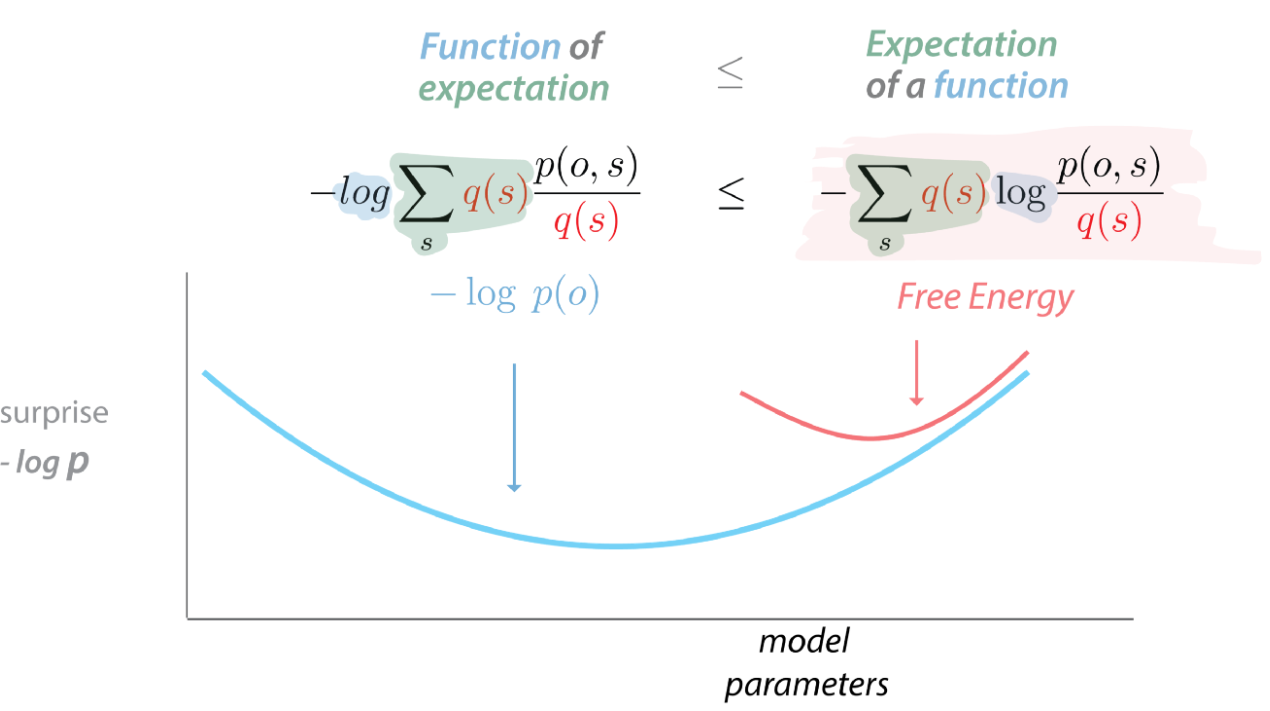
\includegraphics[width=0.7\linewidth]{ten}}
		\label{ris:image}
	\end{figure}
	%\vspace{-3mm}
	
	Мы можем пойти на шаг дальше и убрать минус перед логарифмом. Это приведет нас к определению, которое используют в статьях про Активный Вывод[Active Inference]:
	
	%\vspace{-3mm}
	\begin{figure}[h]
		\centering{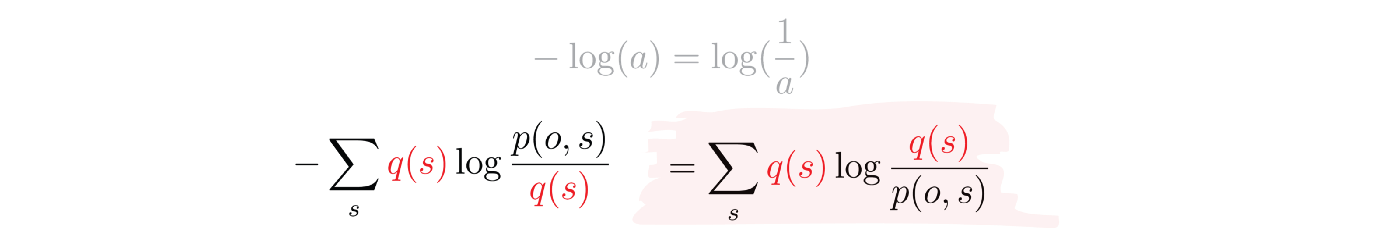
\includegraphics[width=0.5\linewidth]{eleven}}
		\label{ris:image}
	\end{figure}
	%\vspace{-3mm}
	
	Крутая вещь в Свободной Энергии заключается в том, что веса в суммировании определяются \textbf{q(s)}, и мы имеем полный контроль над $q(s)$. Получается, что мы можем покачивать $q(s)$ таким образом, чтобы минимизировать свободную энергию.
	
	Используя пару стандартных идентификаторов, Свободная Энергия[Free Energy] (обычно добавляемая в литературе как «Variational») может быть разложена двумя эквивалентными способами.
	
	%\vspace{-3mm}
	\begin{figure}[h]
		\centering{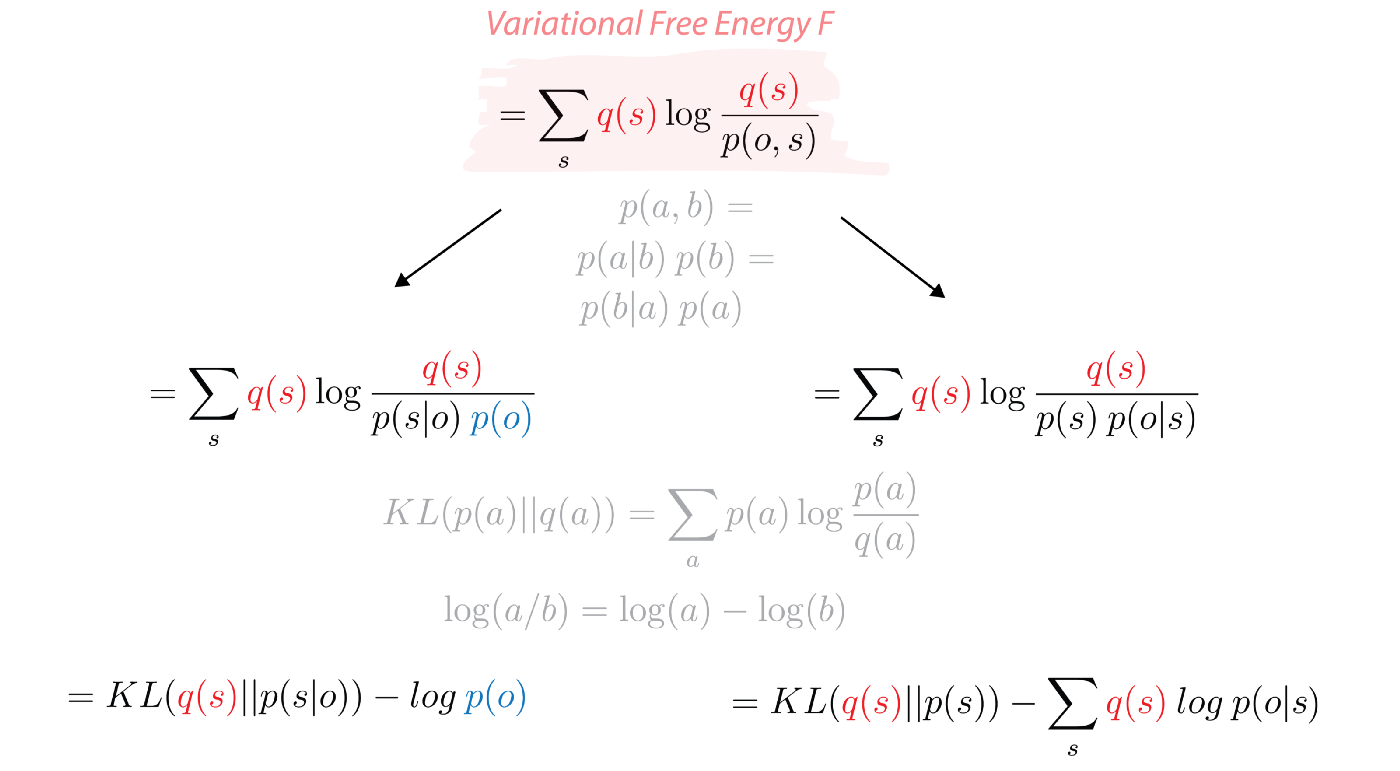
\includegraphics[width=0.8\linewidth]{twelve}}
		\label{ris:image}
	\end{figure}
	%\vspace{-3mm}
	
	Хотя правая ветвь обычно используется на практике, давайте сосредоточимся на левой, так как она дает нам хорошее теоретическое понимание [примечание: мы можем убрать ожидание (сумму по s из $q(s)$) перед $-log$ $p(o)$, поскольку $p(o)$ не зависит от s, а $q(s)$ как распределение вероятностей суммируется до 1]. Это говорит о том, что свободная энергия равна дивергенции KL (Кульбака - Лейблера) между $q(s)$ и $p(s|o)$, и сюрпризу $-log$ $p(o)$.
	
	%\vspace{-3mm}
	\begin{figure}[h]	
		\centering{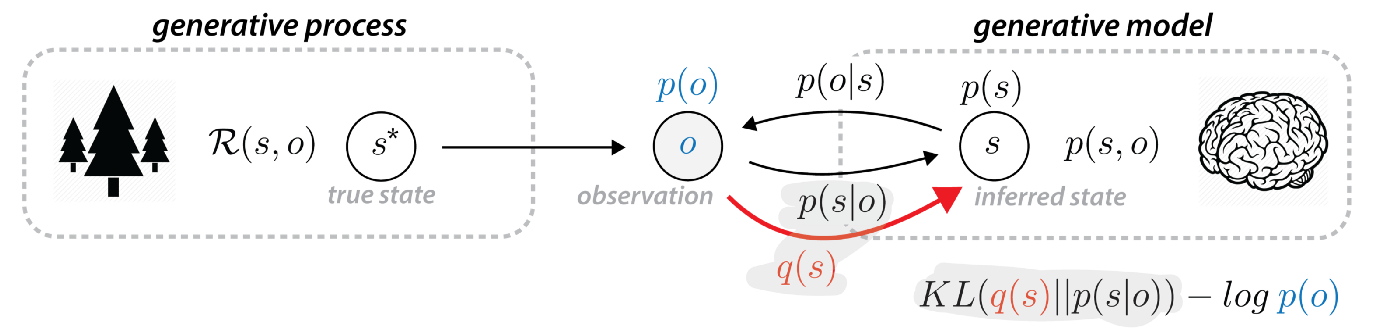
\includegraphics[width=0.8\linewidth]{thirteen}}
		\label{ris:image}
	\end{figure}
	%\vspace{-3mm}
	
	Таким образом, минимизируя свободную энергию, произвольное распределение $q(s)$ становится ближе к постериорному $p(s|o)$, и если они совпадают, дивергенция KL становится равной 0, а свободная энергия точно равна неожиданности[surprise]. Таким образом, чем больше мы минимизируем свободную энергию путем покачивания $q(s)$, тем ближе она становится к неожиданности[surprise] (поскольку это верхняя граница), а путем минимизации свободной энергии путем, покачивания параметров $p(o,s)$ мы можем минимизировать неожиданность[surprise] еще больше. Это подробно показано в  \href{https://medium.com/@solopchuk/intuitions-on-predictive-coding-and-the-free-energy-principle-3fc5bcedc754}{посте о прогнозирующем кодировании[pedictive coding]}, которое является следствием принципа свободной энергии, применяемого к восприятию. Вот краткое изложение на данный момент: минимизируем приближение к неожиданности (свободную энергию) $\Rightarrow$ избегаем неожиданных наблюдений $\Rightarrow$ избегаем неожиданных состояний[states] $\Rightarrow$ поддерживаем гомеостазис $\Rightarrow$ остаемся живыми.
	
	До сих пор мы имели дело со статической ситуацией, с одним скрытым состоянием и одним набором наблюдений, но реальный мир динамичен. Таким образом, у нас будет скрытое состояние в каждый момент времени, и, поскольку все имеет тенденцию зависеть от того, \textbf{что произошло раньше}, мы будем предполагать, что s в определенный момент времени t зависит от s в предыдущий момент времени. Например, вероятность увидеть радугу напрямую зависит от того, шел ли дождь раньше.
	
	%\vspace{-3mm}
	\begin{figure}[h]	
		\centering{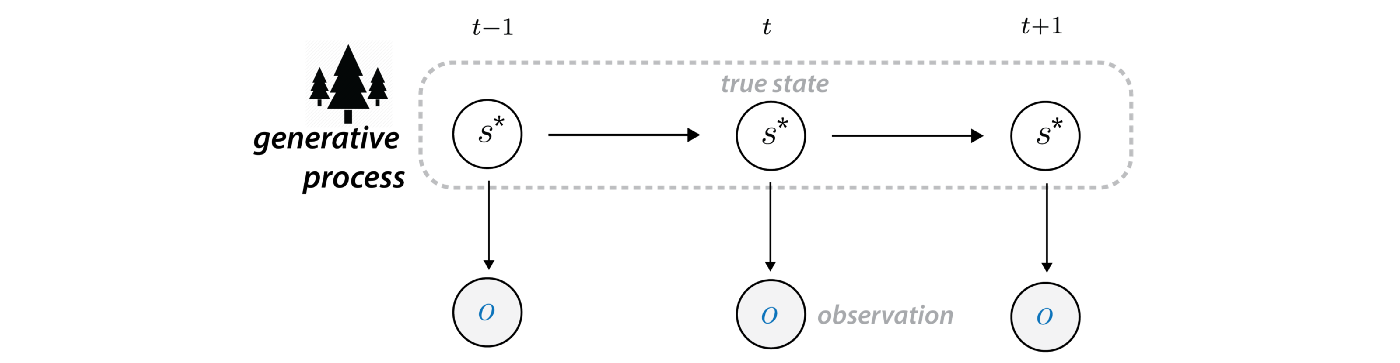
\includegraphics[width=0.5\linewidth]{fourteen}}
		\label{ris:image}
	\end{figure}
	%\vspace{-3mm}
	
	Как и прежде, мы пытаемся смоделировать истинный генерируемый процесс[true generative process], изучая генерируемую модель[generative process] $p(o,s)$ и получая приближение к постериорным $q(s)$ на каждом временном шаге. Как и в простой статической ситуации, мы можем найти, каким образом нужно изменить параметры $p(o,s)$ и $q(s)$, чтобы уменьшить свободную энергию, а затем сделать много маленьких шагов в этом направлении.

	%\vspace{-3mm}
	\begin{figure}[h]	
		\centering{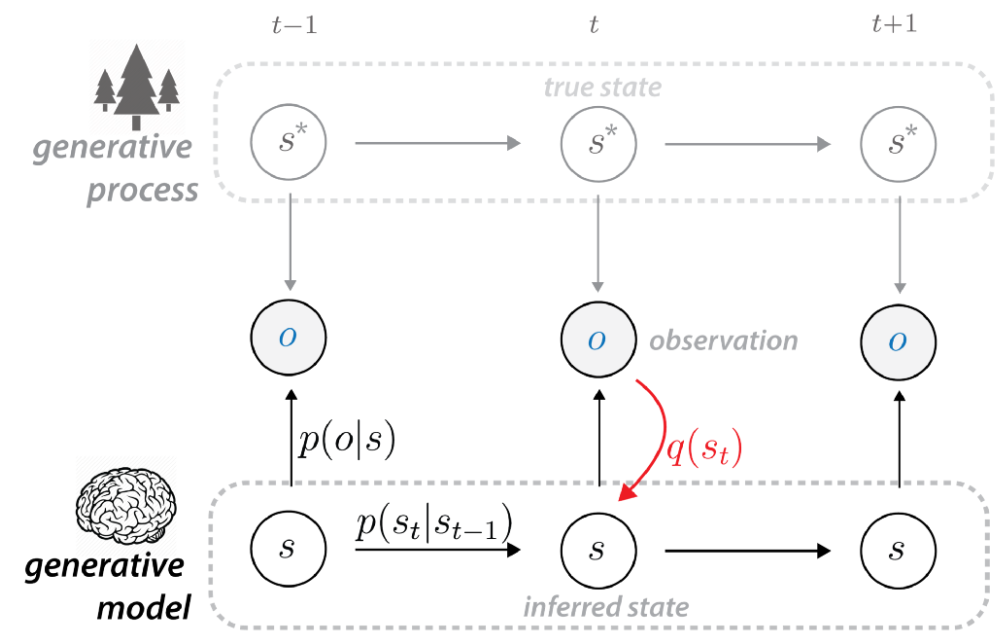
\includegraphics[width=0.5\linewidth]{fifteen}}
		\label{ris:image}
	\end{figure}
	%\vspace{-3mm}
	
	Это будет работать, но мы просто будем пассивно наблюдать за окружающей средой. Что если мы тоже будем воздействовать на нее? В этом случае s в определенный момент времени t будет зависеть от s в предыдущий момент времени и нашего действия u. Другими словами, действие может напрямую влиять на состояние мира, поэтому другое действие может привести к иному будущему (например, мы можем физически двигать вещи своими действиями).

	%\vspace{-3mm}
	\begin{figure}[h]	
		\centering{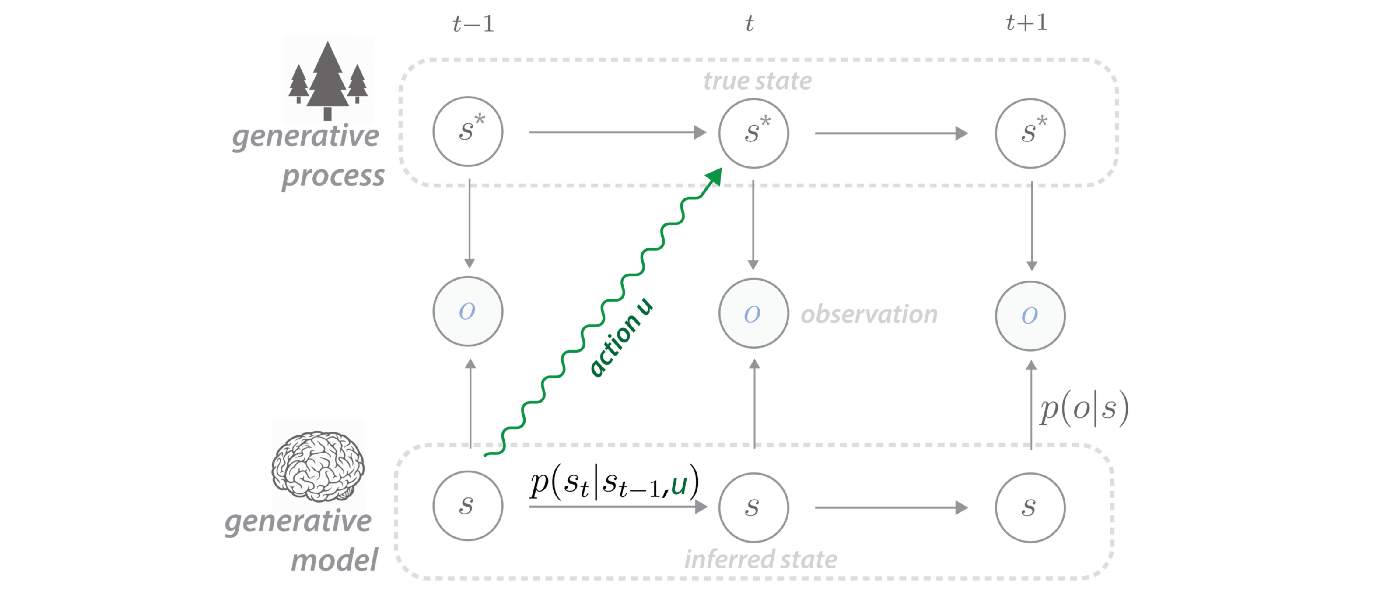
\includegraphics[width=0.5\linewidth]{sixteen}}
		\label{ris:image}
	\end{figure}
	%\vspace{-3mm}
	
	Теперь вывод становится активным [inference becomes active]! Нам просто нужно найти способ выбрать хорошее действие на каждом временном шаге. В действительности кажется, что мы не рассматриваем последствия действий только на следующем временном шаге. Мы планируем всю политику, серию действий, ориентированных на отдаленные во времени цели. Поэтому, если есть много возможных действий и много будущих моментов времени $\Rightarrow$ есть много потенциальных политик, которые мы можем предпринять. Активный вывод говорит: просто рассмотрите все варианты. Таким образом, мы делаем вывод, аппроксимируя $p(s|o)$ с $q(s)$ одновременно (параллельно) для каждой возможной политики $\pi$.

	%\vspace{-3mm}
	\begin{figure}[h]	
		\centering{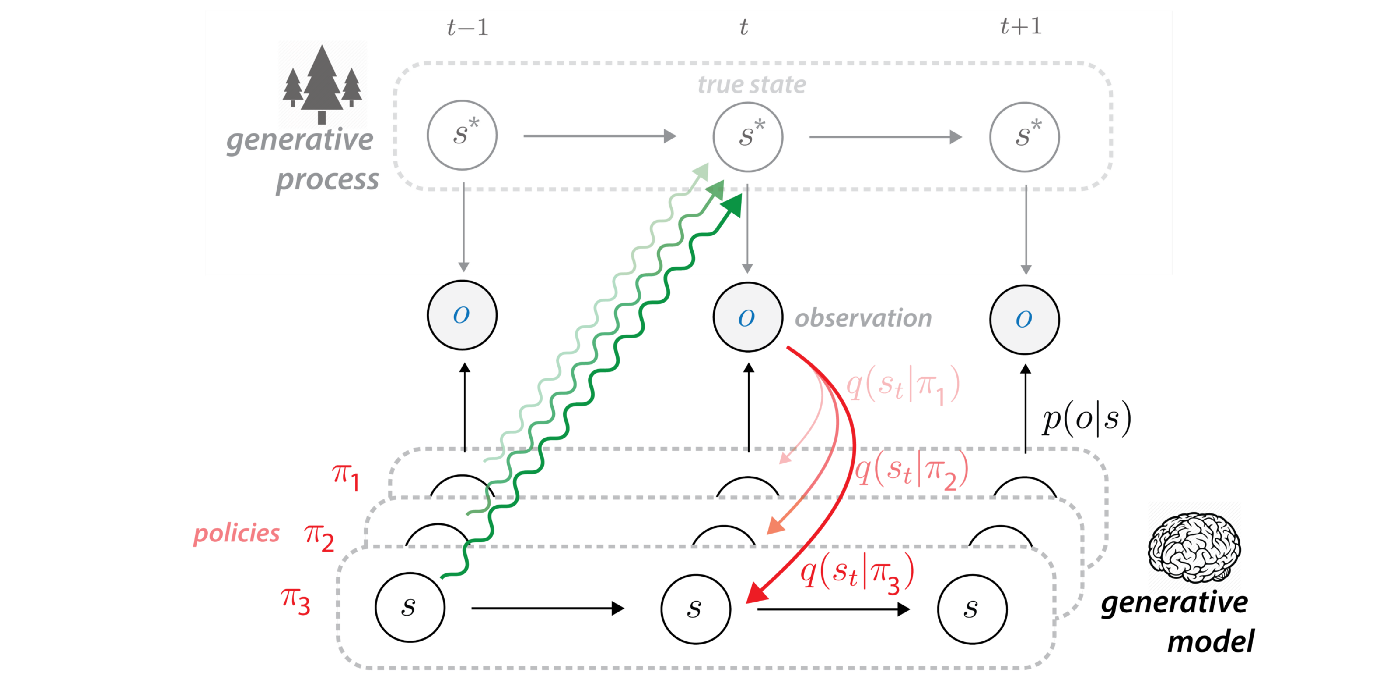
\includegraphics[width=0.6\linewidth]{seventeen}}
		\label{ris:image}
	\end{figure}
	%\vspace{-3mm}
	
	И поскольку наша цель остается прежней - минимизировать неожиданность[surprise] путем минимизации свободной энергии[free energy] - мы можем вычислить свободную энергию[free energy] (и направление изменения $q(s)$, которое минимизирует FE) при каждом возможном шаге политики и времени.
	
	\textbf{Политики(имеется в виду планы)[Policies], которые минимизируют Свободную Энергию[Free Energy] в будущем, являются предпочтительными}. Допустим, мы планируем на 10 временных шагов вперед. Если мы находимся в момент времени t = 1, для каждой политики мы суммируем Свободные энергии для шагов с 1 по 10 времени и выбираем политику, которая имеет минимальную кумулятивную Свободную энергию в будущем. Давайте еще раз посмотрим на общую картину того, как можно рассчитать свободную энергию:
	
	%\vspace{-3mm}
	\begin{figure}[h]	
		\centering{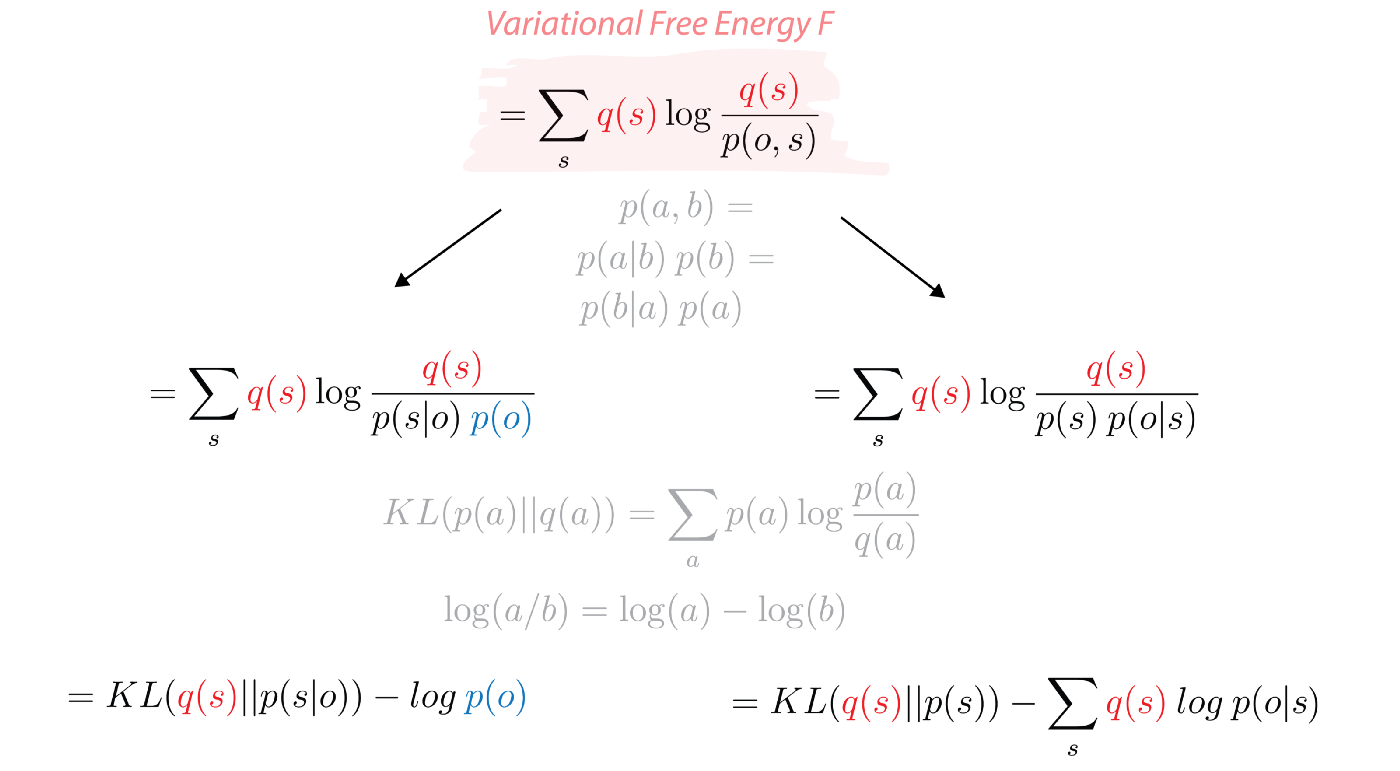
\includegraphics[width=0.7\linewidth]{eightteen}}
		\label{ris:image}
	\end{figure}
	%\vspace{-3mm}
	
	Левая ветвь показывает нам важные теоретические свойства минимизации свободной энергии (например, что $q(s)$ приближается к $p(s|o)$), но это нецелесообразно, поскольку мы используем свободную энергию для аппроксимации $-log$ $p(o)$ в первую очередь. Итак, давайте посмотрим на правую ветвь, которая является стандартным способом вычисления свободной энергии:
	
	%\vspace{-3mm}
	\begin{figure}[h]	
		\centering{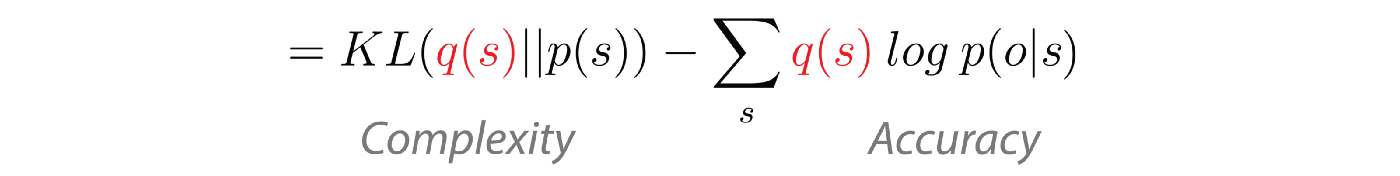
\includegraphics[width=0.4\linewidth]{nineteen}}
		\label{ris:image}
	\end{figure}
	%\vspace{-3mm}
	
	Эти два термина обычно называют сложностью[complexity] и точностью[accuracy]. Сложность[Complexity] показывает, насколько аппроксимация апостериорного $q(s)$ отклоняется от приорного $p(s)$, и количественно определяет, сколько дополнительных битов информации, которых нет в приорном распределении, мы хотим закодировать в приблизительном апостериорном $q(s)$. Точность[Accuracy] (ожидаемое значение $p(o|s)$) оценивает вероятность того, что состояниям дан конкретный результат o. Хотя мы можем легко вычислить Сложность[Complexity], существует проблема в оценке Точности[Accuracy] для будущих временных шагов - просто потому, что мы еще не наблюдали результаты. Таким образом, нам нужен другой способ вычисления свободной энергии[free energy], поэтому мы пойдем по левой ветви разложения FE. Но здесь есть одна загвоздка: поскольку у нас нет доступа к будущим наблюдениям - нам нужно угадать, как они могли бы выглядеть, и взять взвешенную сумму свободной энергии по догадкам $p(o|s)$. Обратите внимание, что мы будем ставить вероятности на $\pi$, так как свободная энергия оценивается отдельно для каждой политики. Предполагается, что только отображение наблюдения состояния $p(o|s)$ одинаково для всех политик.
	
	%\vspace{-3mm}
	\begin{figure}[h]	
		\centering{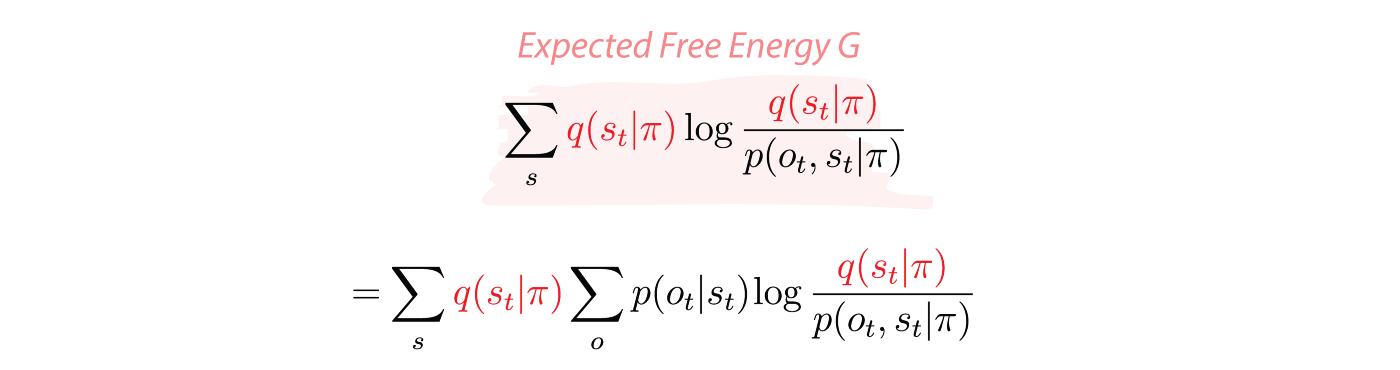
\includegraphics[width=0.4\linewidth]{twenty}}
		\label{ris:image}
	\end{figure}
	%\vspace{-3mm}
	
	Итак, нам нужно предсказывать как будущие состояния $q(s|\pi)$, так и наблюдения. А также оценивать свободную энергию на их основе. Давайте пройдем шаг за шагом, сначала сосредоточившись на знаменателе $p(o,s|\pi)$. Рассматривая левую ветвь разложения свободной энергии, показанную выше, мы можем преобразовать ее так же, как $p(s|o) \cdot p(o)$:
	
	%So we will have to predict both future states q(s|pi) and observations, and to estimate the Free Energy based on that. Let's go step by step, first focusing on the denominator p(o, s|pi). Following the left branch of Free Energy expansion shown above, we can split it as p(s|o) p(o):
	
	%\vspace{-3mm}
	\begin{figure}[h]
		\centering{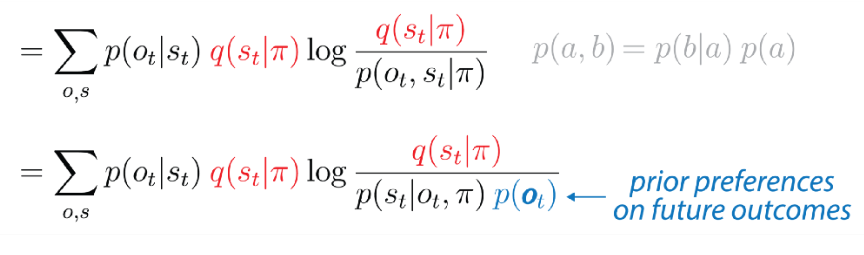
\includegraphics[width=0.7\linewidth]{1.png}}
	\end{figure}
	%\vspace{-3mm}
	
	$p(o)$ - это априорные предпочтения относительно будущих наблюдений [the prior preference on the future outcomes] (которые пропорциональны вознаграждению в классическом обучении с подкреплением). Разделив логарифм, мы получаем следующие две величины:  отрицательное эпистемическое (т.е. знание) значение [negative epistemic value] и ожидаемое предшествующее предпочтение [expected prior preference]:
	
	%The term p(o) is the prior preference on the future outcomes (which is proportional to reward in classical reinforcement learning). We will see how it will play out later. Splitting the log, we get the following 2 terms — negative epistemic (i.e. knowledge) value and expected prior preference:
	
	%\vspace{-3mm}
	\begin{figure}[h]
		\centering{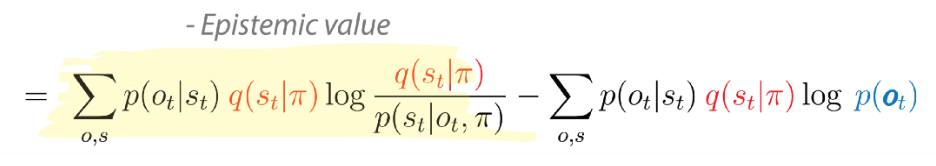
\includegraphics[width=0.7\linewidth]{2.png}}
	\end{figure}
	%\vspace{-3mm}
	
	Короче говоря, эпистемическое значение [epistemic value] говорит нам, насколько будущие наблюдения могут уменьшить нашу неопределенность относительно аппроксимации апостериорного $q(s)$ [the approximate posterior q(s)]. Давайте сначала закончим вывод, а затем обсудим его подробно. У нас есть истинное апостериорное $p(s|o,\pi)$ в знаменателе левого слагаемого, которое, как мы знаем, трудно вычислить, особенно в будущем (имейте в виду, что мы предсказываем будущие состояния и наблюдения). Таким образом, мы могли бы применить формулу Байеса, чтобы повторно выразить это соотношение в более вычислимых выражениях:
	
	%In brief, epistemic value tells us how much future observations can decrease our uncertainty over the approximate posterior q(s). Let's finish the derivation first and then discuss it in detail. We have the true posterior p(s|o,pi) in the denominator of the left term, which we know is hard to compute, especially in the future (keep in mind that we are predicting future states and observations). So we could apply Bayes formula to re-express that ratio in more computable terms:
	
	%\vspace{-3mm}
	\begin{figure}[h]
		\centering{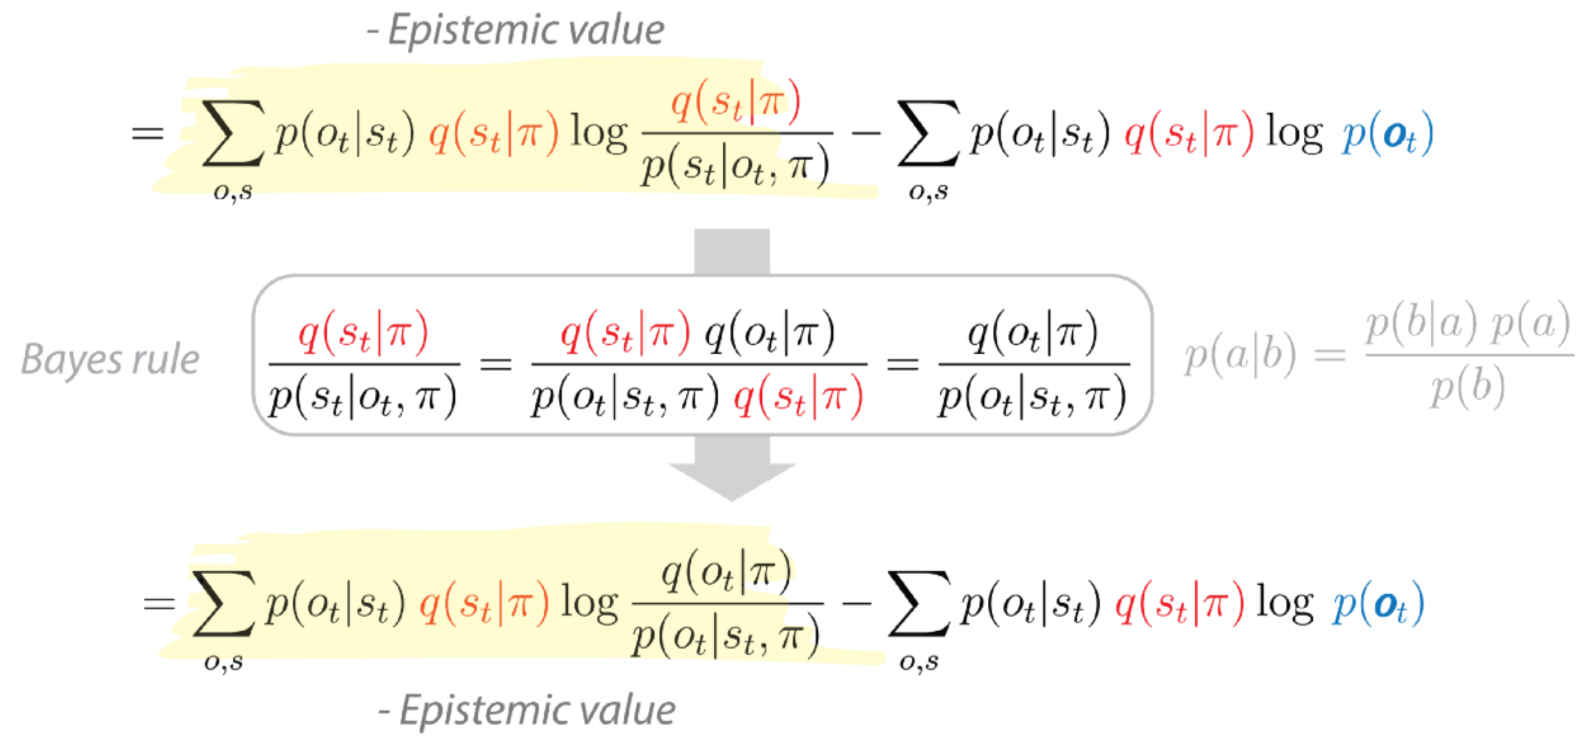
\includegraphics[width=0.8\linewidth]{3.png}}
	\end{figure}
	%\vspace{-3mm}
	
	Это было бы легче сделать, если бы вы пренебрегли зависимостью от $\pi$. Тогда $q(o)$ это вроде маргинального распределения (marginal likelihood), $p(o|s)$ -- вероятность [likelihood] и $q(s_t|\pi)$ -- априорное распределение (?). Вы также можете заметить, что для некоторых распределений <<$p$>> заменяется на <<$q$>>. Это результат аппроксимации, так как, например, $p(s|o,\pi)$ является истинным апостериорным распределением, которое мы можем аппроксимировать с помощью $q(s|o,\pi)$, что при разложении приведет к тому, что все компоненты формулы Байеса будут формой $q$. Также обратите внимание, что $q(o|s,\pi)$ это то же самое, что и $p(o|s,\pi)$, поскольку это все еще относится к той же вероятности [likelihood].
	
	%It could be easier to follow if you disregard the dependence on pi. Then, q(o) is like marginal likelihood, p(o|s) is the likelihood, and q(s_t|pi) is the prior. You may also notice that ‘p’s get interchanged with ‘q’ for some distributions. This is a result of approximations, since, for example, p(s|o,pi) is a true posterior distribution which we can approximate with q(s|o,pi), which, when expanded, would yield all components of Bayes formula to be q. Also note that q(o|s,pi) is the same as p(o|s,pi) since it’s still referring to the same likelihood.
	
	Мы также могли бы объединить логарифмы и снова разделить их по-другому, что приводит нас к окончательной форме ожидаемой свободной энергии:
	
	%We could also combine the logs and split again in a different way which brings us to the final form of expected Free Energy:
	
	%\vspace{-3mm}
	\begin{figure}[h]
		\centering{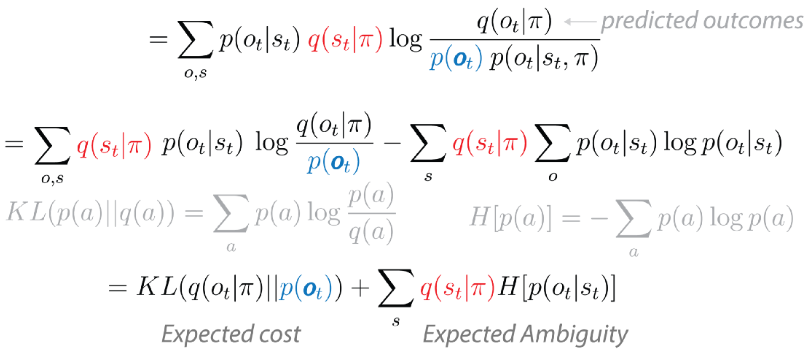
\includegraphics[width=0.8\linewidth]{4.png}}
	\end{figure}
	%\vspace{-3mm}
	
	Примечание: на левой стороне мы можем повторно выразить $q(s|\pi) p(o|s)$ как совместное распределение $q(s,o)$ и просуммировать по всем $s$, чтобы получить $q(o)$. Это даст нам ожидаемую дивергенцию Кульбака-Лейблера. А на правой стороне мы можем удалить $\pi$ из $p(o|s,\pi)$, потому что вероятность [likelihood] одинакова для каждой политики.
	
	%note: on the left side, we can re-express q(s|pi) p(o|s) as a joint q(s,o), and marginalize s to get q(o), giving us the expected KL divergence; and on the right side, we can remove pi from p(o|s,pi) because likelihood is the same for every policy
	
	Левое слагаемое (называемое "Издержки" или "Риск") -- это дивергенция Кульбака-Лейблера между двумя распределениями: ожидаемыми в рамках политики $\pi$ наблюдениями $q(o|\pi)$ и априорными предпочтениями [prior preferences]. Таким образом, минимизация ожидаемой свободной энергии будет способствовать политике, которая приведет к наблюдениям, которые нам нравятся. И правое слагаемое, неоднозначность [Ambiguity], количественно определяет, насколько неопределенным является отображение между состоянием и наблюдениями $p(o|s)$. И это окончательная формула свободной энергии в будущем. Давайте теперь посмотрим на эпистемическое значение (слагаемое, которое появилось раньше, окрашено в желтый цвет).
	
	%The left term (called 'Cost' or 'Risk') is the KL divergence between 2 distributions: expected observations under the policy pi q(o|pi) and prior preferences. So minimizing expected Free Energy would favor policies that will result in observations we like. And the right term, Ambiguity, quantifies how uncertain is the mapping between state and observations p(o|s). And this is the final formula of Free Energy in the future. Let's look on epistemic value now (the term that appeared earlier, colored in yellow).
	
	Эпистемическое значение говорит нам, как много мы могли бы извлечь из окружающей среды, если бы следовали этой политике. Так происходит потому, что эпистемическое значение представляет собой взаимную информацию [mutual information] между скрытыми состояниями $s$ и ожидаемыми наблюдениями $o$. Взаимная информация количественно определяет, насколько неопределенность ($H$) по одной переменной уменьшается, если мы знаем другую.
	
	%Epistemic value tells us how much we could learn from the environment if we followed this policy. This is because epistemic value is a mutual information between the hidden states s and expected observations o. And mutual information quantifies how much uncertainty (H) over one variable decreases if we know the other.
	
	%\vspace{-3mm}
	\begin{figure}[h]
		\centering{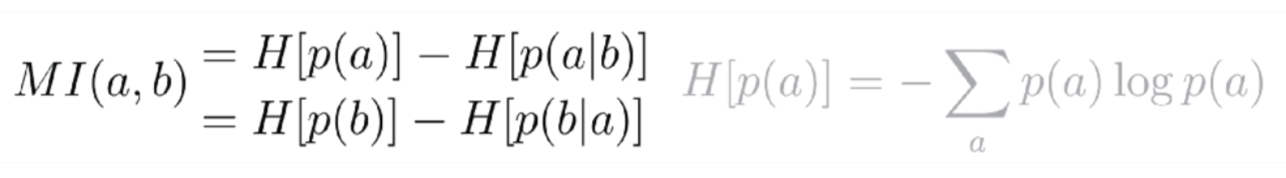
\includegraphics[width=0.7\linewidth]{5.png}}
	\end{figure}
	%\vspace{-3mm}
	
	Аналогично, взаимная информация может быть повторно выражена как дивергенция Кульбака-Лейблера между совместным распределением двух переменных (если взаимная информация велика, то знание одной переменной говорит нам много о распределении другой) и произведением их маргинальных плотностей [marginals] (как если бы они были полностью независимы). Нам просто нужно перевернуть номинатор и знаменатель (потому что эпистемическое значение отрицательно в уравнениях). Обратите внимание, что мы можем удалить $\pi$ из $p(o|s,\pi)$, потому что вероятность одинакова для каждой политики.
	
	%Equivalently, mutual information can be re-expressed as the KL divergence between a joint distribution of 2 variables (if MI is high, knowing one variable tells us a lot about the distribution of the other) and product of their marginals (as if they were completely independent). We just need to flip nominator and denominator (because epistemic value is negative in the equations). Note, we can remove pi from p(o|s,pi) because likelihood is the same for every policy.
	
	%\vspace{-3mm}
	\begin{figure}[h]
		\centering{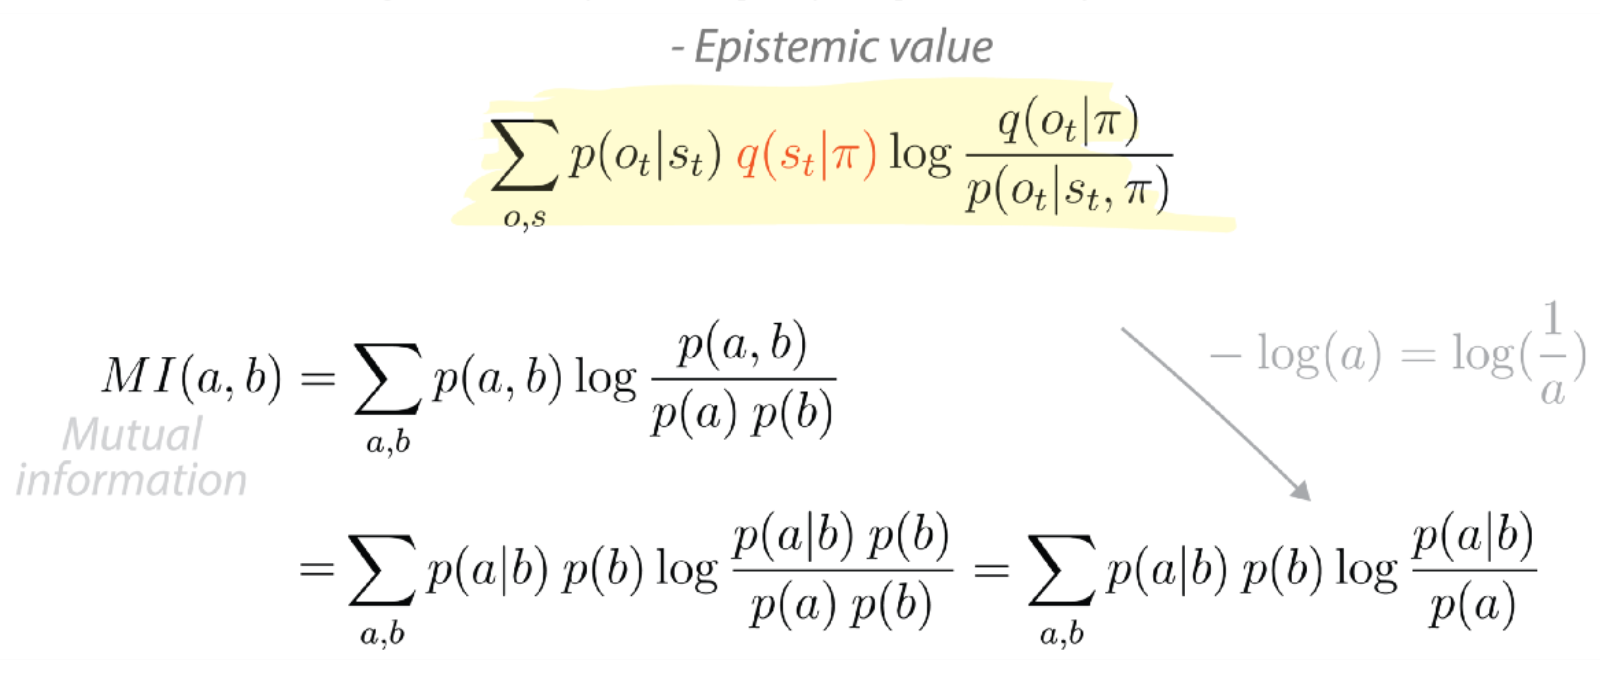
\includegraphics[width=0.7\linewidth]{6.png}}
	\end{figure}
	%\vspace{-3mm}
	
	На практике эпистемическое значение зависит от неопределенности относительно будущих состояний $q(s|\pi)$. Если вы абсолютно уверены, тогда $H[q(s|\pi)]$ невелико, вам больше нечему учиться, поэтому эпистемическая ценность будет низкой. Но если вы не уверены, $H[q(s|\pi)]$ высоко, и существует сильная зависимость между состояниями и наблюдениями (поэтому $H[q(s|o)]$ низок), то взаимная информация будет высокой (см. формулы взаимной информации в терминах энтропий выше). Надеюсь, что прочитав приведенным описаниям несколько раз и пройдя их самостоятельно, оно станет простым.
	
	%Practically, epistemic value depends on the uncertainty about future states q(s|pi). If you are very certain, H[q(s|pi)] is small, there is nothing more to learn, so epistemic value will be low. But if you are uncertain, H[q(s|pi)] is high, and there is a strong dependency between states and observations (so H[q(s|o) is low), then mutual information will be high (see MI formulas in terms of entropies above). Hopefully, going through the passages a few times and deriving them yourself, will make it straightforward. Regarding the interpretations of various Free Energy terms, they are discussed at lengths in the papers.
	
	Вот небольшой пример того, что на самом деле произошло бы в мозгу агента, если бы он использовал активное умозаключение [active inference]. Для простоты предположим, что окружающая среда имеет только два состояния $s$: <<$1$>> и <<$2$>>, например, есть пища в вашем желудке $(1)$ или нет $(2)$. Аналогично, есть только два возможных наблюдения $о$: <<$1$>> и <<$2$>>, вы чувствуете себя сытым $(1)$ или голодным $(2)$. Предположим, что мы уже знаем параметры генеративной модели [generative model] $p(o,s)$. Вероятность (называемая матрицей $A$) $p(o|s)$ сопоставляет состояния с наблюдениями -- если у вас есть еда -- вас кормят и наоборот. Вероятность перехода $p(s_t|s_{t-1},u)$ отображает предыдущее состояние в следующее. Но поскольку переход также зависит от действия u, мы можем выразить его в виде отдельной матрицы переходов ($B$) для каждого действия. Предположим, что мы можем либо пойти за едой ($u_1$), либо ничего не делать ($u_2$). Так что если мы выберем $u_1$ -- у нас будет еда в следующем состоянии, независимо от того, есть ли она у нас сейчас, и наоборот. Наконец, у нас также есть предварительные предпочтения $p(o)$ -- мы любим, чтобы нас кормили и не голодали, поэтому мы приписываем более высокую вероятность наблюдению <<$1$>> -- кормили. Другими словами, Мы выражаем предпочтения по отношению к наблюдениям как вероятность $p(o)$.
	
	%\vspace{-3mm}
	\begin{figure}[h]
		\centering{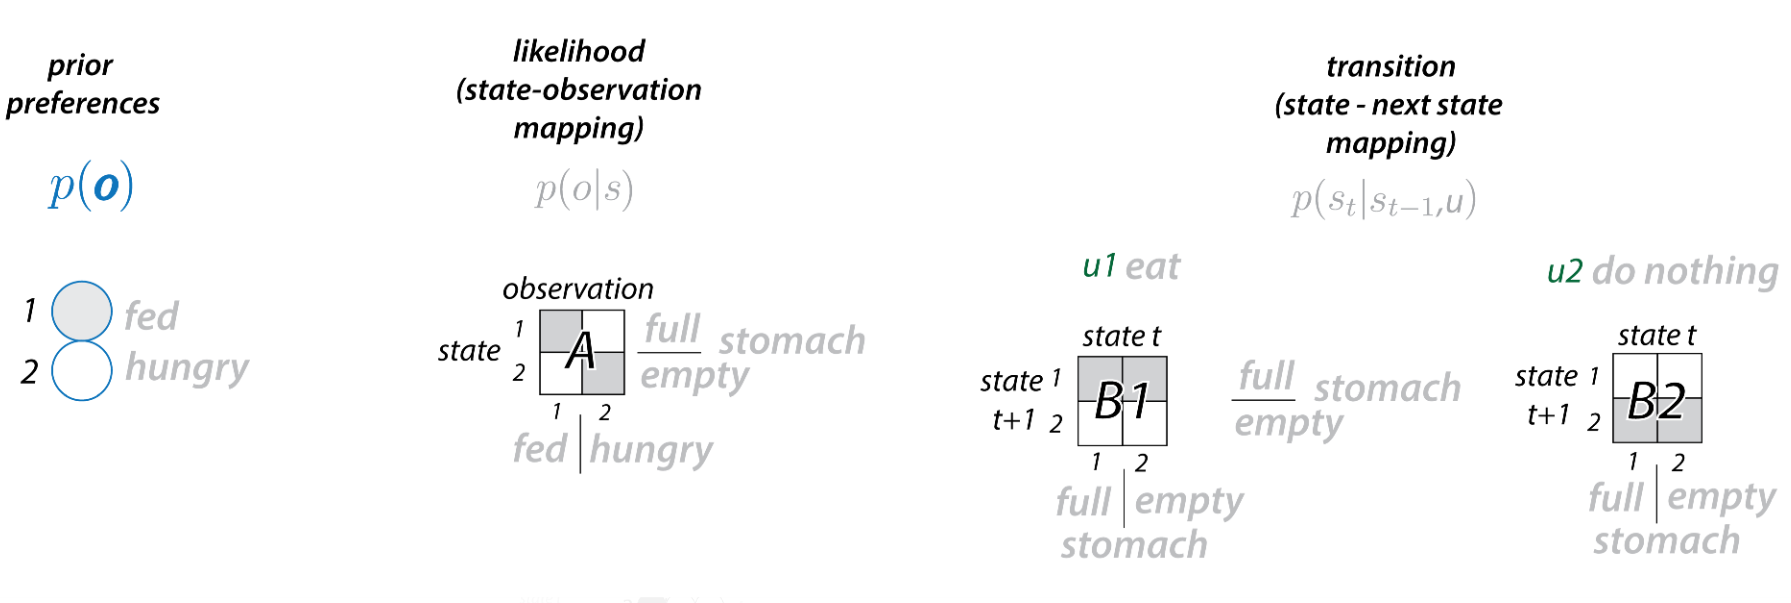
\includegraphics[width=0.9\linewidth]{7.png}}
	\end{figure}
	%\vspace{-3mm}
	
	%Here is a minimalistic example of what would actually happen inside agent's brain, if it were to use active inference. For simplicity, suppose the environment has only two states s : "1" and "2", for example, there is food in your stomach (1) or not (2). Similarly, there are only two possible observations o: "1" and "2", you feeling fed (1) or hungry(2). Suppose we already know the parameters of the generative model p(o,s). The likelihood (called "A" matrix) p(o|s) maps states to observations — if you have food — you are fed and vice versa. The transition probability p(s\_t|s\_t-1,u) maps the previous state to the next one. But since the transition also depends on action u, we can express it as a separate transition matrix ("B") for each action. Suppose we can either go get food (u1) or do nothing (u2). So if we pick u1 — we will have food in the next state, regardless of whether we have it now, and vice versa. Finally, we also have prior preferences p(o) — we like to be fed and not hungry, so we assign a higher probability to observation "1" — fed. In other words, we express preferences over observations as probability p(o).
	
	Теперь представьте, что мы наблюдаем, что мы голодны, и должны планировать свои действия на два шага вперед.
	
	%\vspace{-3mm}
	\begin{figure}[h]
		\centering{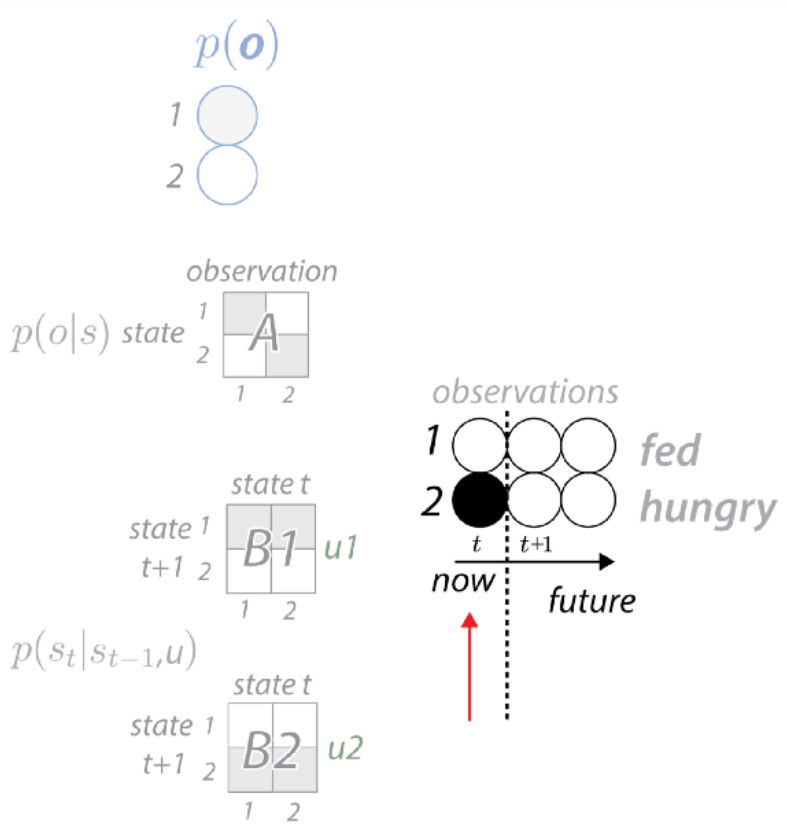
\includegraphics[width=0.4\linewidth]{8.png}}
	\end{figure}
	%\vspace{-3mm}
	
	%Now imagine we observe that we are hungry and have to plan our actions for the next 2 time steps.
	
	Поскольку есть только два возможных действия и два шага, мы можем оценить все возможные политики: $1-1$ (идти за едой оба раза), $1-2$, $2-1$, $2-2$. На самом деле мы будем оценивать апостериорное распределение по будущим состояниям (будет ли пища находиться в нашем желудке), при каждой из этих политик:
	
	%\vspace{-3mm}
	\begin{figure}[h]
		\centering{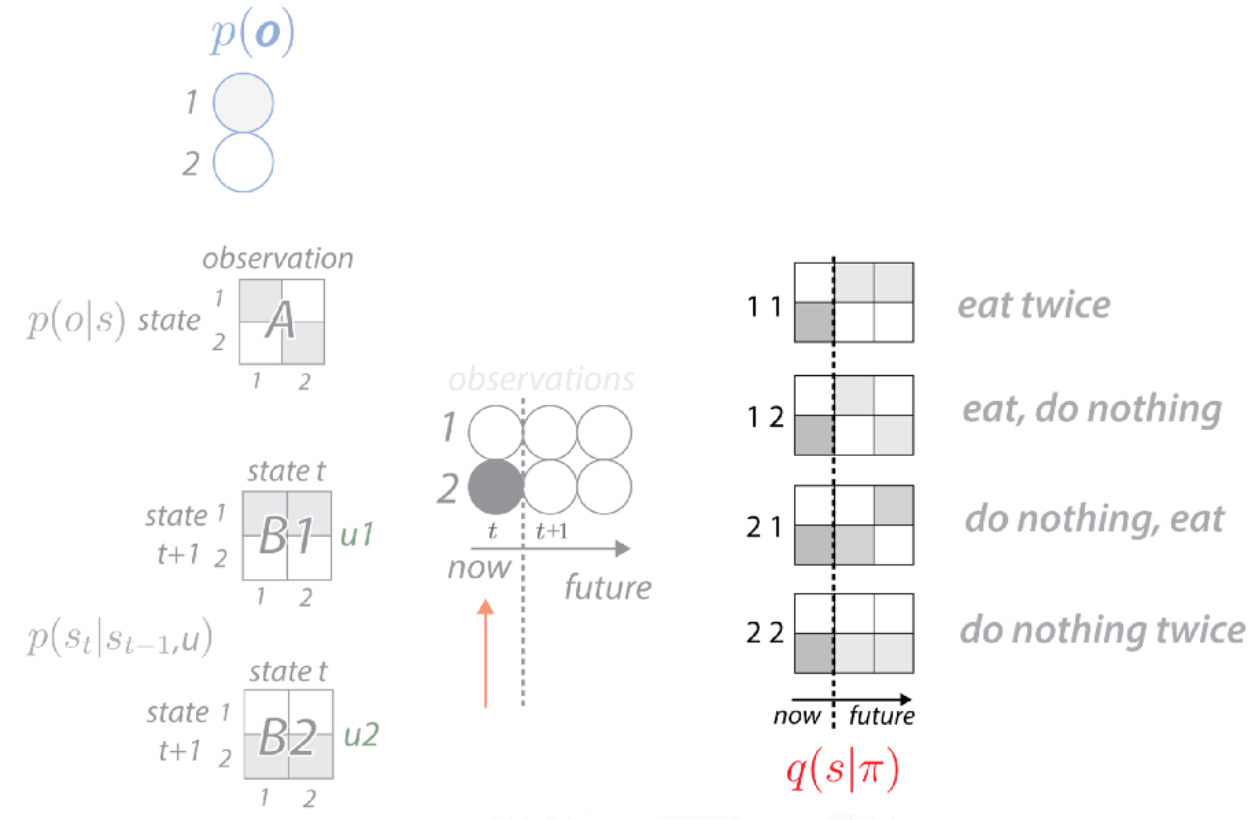
\includegraphics[width=0.8\linewidth]{9.png}}
	\end{figure}
	%\vspace{-3mm}
	
	%Since there are only 2 possible actions and 2 time steps, we can evaluate all possible policies: 11 (go for food in both time steps), 12, 21, 22. In fact we will estimate the posterior distribution on the future states (whether the food will be in our stomach), under each of these policies:
	
	Поскольку мы знаем, как состояния связаны с наблюдениями ($p(o|s)$, матрица $A$), мы можем оценить прогнозируемое наблюдение для каждой политики $q(o|\pi)$ и вычислить дивергенцию Кульбака-Лейблера (заштрихована синим цветом) ожидаемой свободной энергии (??). Аналогично, мы также можем оценить неоднозначность [Ambiguity] (заштрихована оранжевым цветом), который зависит от $p(o|s)$:
	
	%\vspace{-3mm}
	\begin{figure}[h]
		\centering{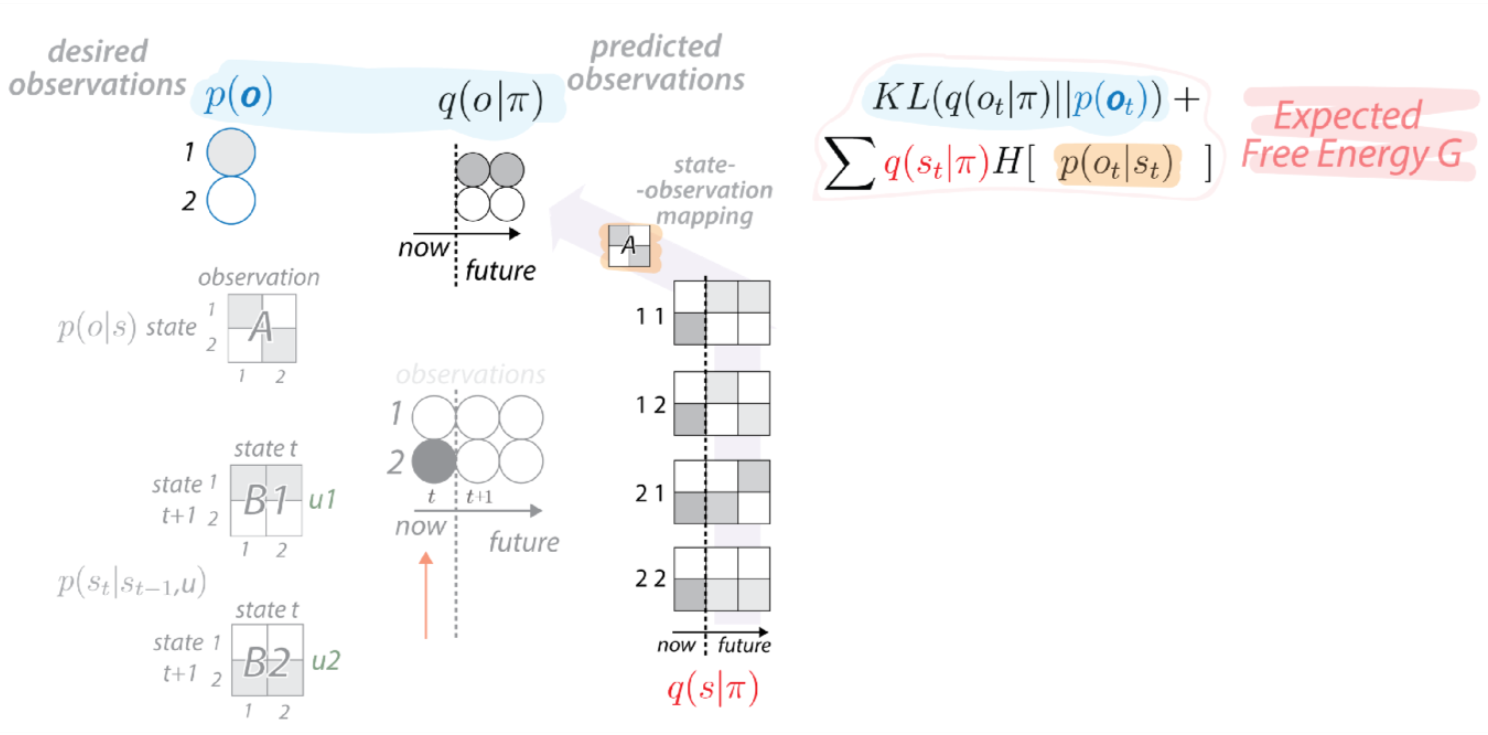
\includegraphics[width=0.8\linewidth]{10.png}}
	\end{figure}
	%\vspace{-3mm}
	
	%Since we know how the states are related to observations (p(o|s), 'A' matrix), we can estimate the predicted observation for each policy q(o|pi), and compute the KL term (shaded in blue below) of the expected Free Energy. Similarly, we can also evaluate the Ambiguity term (shaded in orange below), which depends on p(o|s):
	
	Затем мы суммируем ожидаемую свободную энергию по будущим действиям и преобразуем ее в распределение вероятностей для политики [probability distribution over policy] $q(\pi)$. Так что чем меньше свободная энергия, тем выше вероятность проведения политики. Интересно, что при преобразовании свободная энергия взвешивается (умножается) на точность [precision], которая определяет, насколько мы уверены в своих убеждениях по отношению к политике (то есть, изменяя точность до ее крайних значений, наши убеждения могут разрушаться на одной политике или распространяться равномерно [our beliefs can collapse on a single policy or spread uniformly]). Это важно для определения исследования/эксплуатации [exploration/exploitation], так как чем больше вы уверены в том, что у вас есть хорошая политика (т. е. высокая точность), тем меньше вы исследуете и наоборот.
	
	%\vspace{-3mm}
	\begin{figure}[h]
		\centering{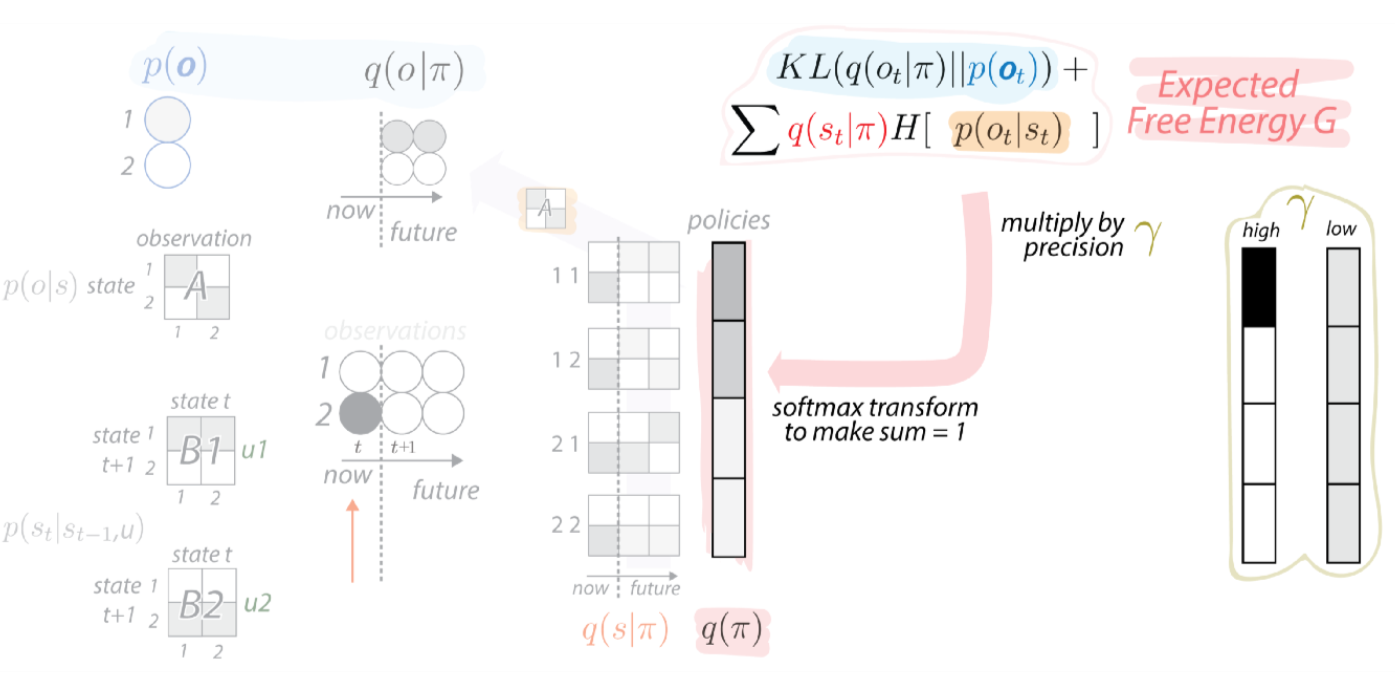
\includegraphics[width=0.8\linewidth]{11.png}}
	\end{figure}
	%\vspace{-3mm}
	
	%Then, we'd sum the expected Free Energy over future time steps and transform it into a probability distribution over policy q(pi). So the smaller the Free Energy — the higher the probability of the policy. Interestingly, during the transformation, Free energy is weighted (i.e. multiplied) by precision, that determines how much we are confident about the beliefs over policies (i.e. by changing precision to its extrmes, our beliefs can collapse on a single policy or spread uniformly). This is imporant to determine exploration/exploitation, as the more confident you are that you have a good policy (i.e. high precision), the less you explore and vice versa.
	
	Теперь вы можете просто выбрать политику, которая максимально минимизирует (?) свободную энергию, но есть более аккуратный способ: вместо выбора 1 политики мы будем делать усреднение по ним. Подумайте об этом так, как если бы в определенный момент времени существовала одна политика, которая давала бы самую низкую свободную энергию, а другие политики были бы просто немного хуже. По мере того как вы будете получать новые наблюдения с течением времени, может оказаться, что лучшая в мире политика была среди тех, которые были "немного хуже" раньше. Но что делать, если вы уже выбрали действие, которое не позволяет вам следовать этой недавно обнаруженной политике? Таким образом, мы позволяем каждой политике голосовать во время выбора действий, причем политики, которые максимально минимизируют свободную энергию, имеют наибольший вес. Мы берем математическое ожидание $q(s|\pi)$ при известном $q(\pi)$ [expectation of $q(s|\pi)$ under $q(\pi)$] -- взвешенная сумма, где веса определяются вероятностью каждой политики. Это приводит к маргинальному распределению $q(s)$, которое неявно включает политику (и, следовательно, ожидаемую свободную энергию).
	
	%\vspace{-3mm}
	\begin{figure}[h]
		\centering{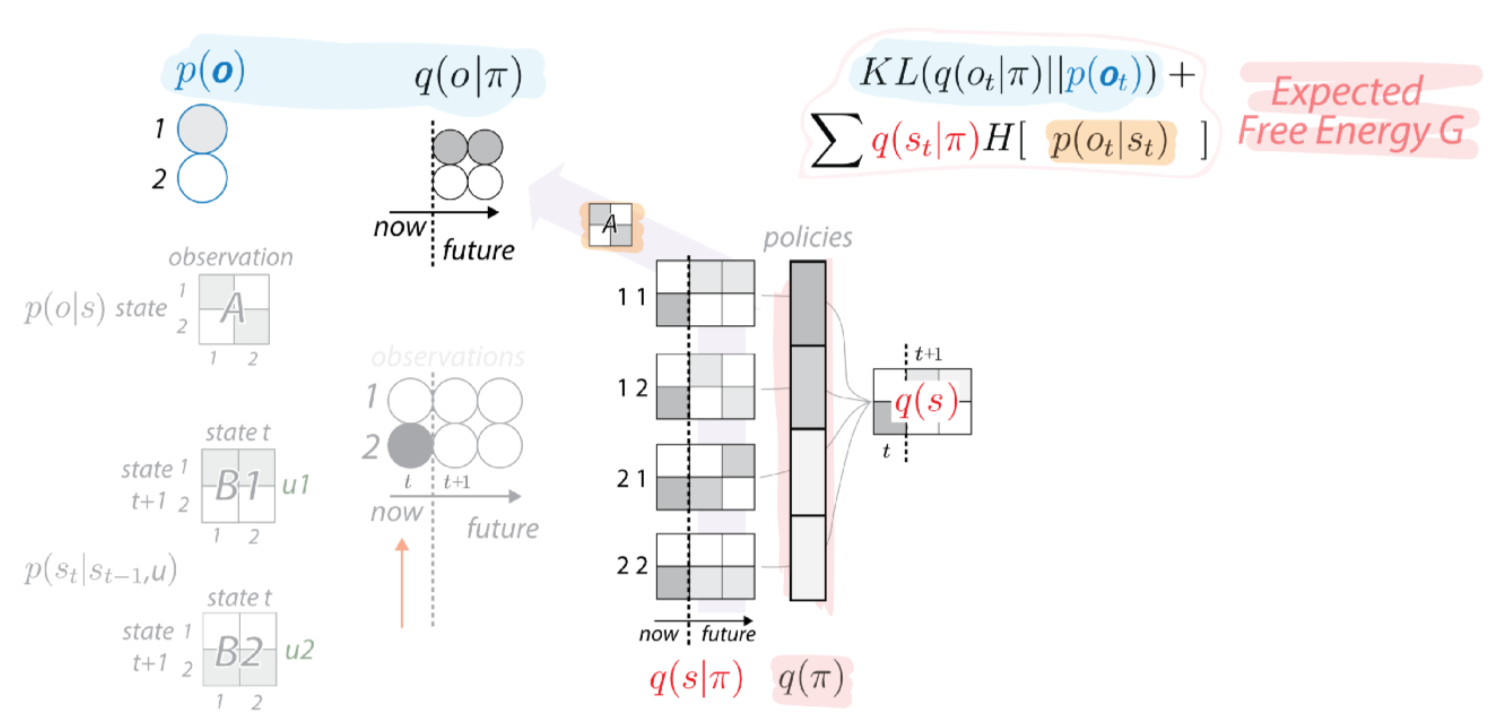
\includegraphics[width=0.7\linewidth]{12.png}}
	\end{figure}
	%\vspace{-3mm}
	
	%Now you could just pick the policy that minimizes Free Energy the most, but, there is a neater way: instead of selecting 1 policy, we would do averaging over them. Think of it as if at a certain time point, there was one policy that would yield the lowest Free Energy, and other policies would be just slightly worse. As you receive new observations over time, it may turn out that the globally best policy was among those that were 'slightly worse' before. But what if you already selected an action that precludes you to follow this newly discovered policy? Thus, we let every policy vote during action selection, with the policies that minimize Free Energy the most, having the biggest weight. We take the expectation of q(s|pi) under q(pi) — a weighted sum, where the weights are defined by the probability of each policy. This results in a marginal distribution q(s), which incorporates the policy (and hence expected FE) implicitly.
	
	И вот теперь мы готовы действовать! Мы выбираем действие, которое минимизирует разницу (дивергенцию Кульбака-Лейблера) между тем, что мы ожидаем увидеть на следующем временном шаге, и тем, что мы должны были бы увидеть, если бы выбрали конкретное действие. Сперва чтобы получить (вероятность) ожидаемых наблюдений, мы умножаем наше убеждение о скрытом состоянии на следующем временном шаге $q(s_{t+1})$ на $p(o|s)$, сопоставляющее состояния и наблюдения (матрица $A$) [by the state-observation mapping p(o|s) ('A' matrix)] :
	
	%\vspace{-3mm}
	\begin{figure}[h]
		\centering{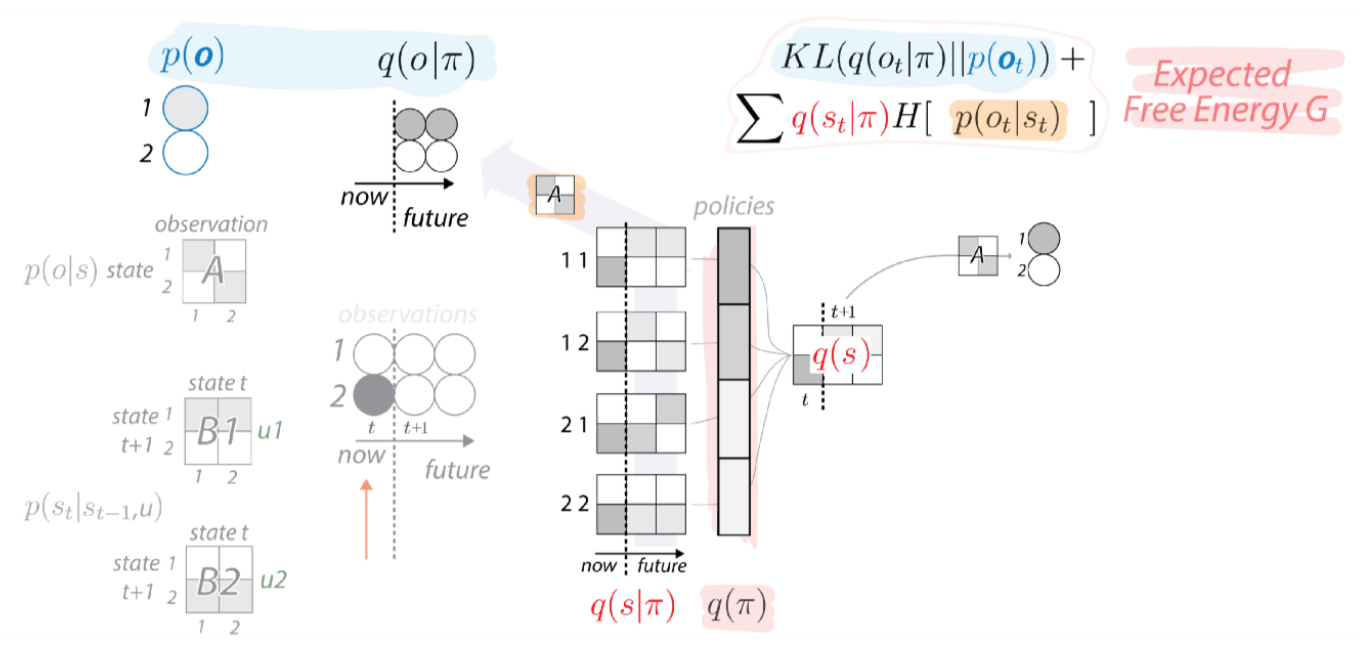
\includegraphics[width=0.7\linewidth]{13.png}}
	\end{figure}
	%\vspace{-3mm}
	
	%And now, we are ready to act! We pick the action that minimizes the difference (KL divergence) of what we expect to see in the next time step, and what we were to see if we picked a specific action. First, to get the (probability of) expected observations, we multiply our belief on the hidden state at the next time step q(s\_t+1) by the state-observation mapping p(o|s) ('A' matrix):
	
	И чтобы получить ожидаемые наблюдения, если мы должны были предпринять определенные действия, мы умножаем нашу веру в скрытое состояние в текущий момент времени $q(s_t)$ на переходную матрицу $B$ для данного действия, чтобы получить гипотетическое следующее состояние, а затем на матрицу $A$, сопоставляющую состояния и наблюдения, чтобы получить гипотетическое наблюдение [And to get the expected observations if we were to take a certain action, we take our belief on the hidden state at the current time step q(s\_t), multiply it by the action-specific state-transition matrix B (to get the hypothetical next state), and then by state-observation matrix A (to get the hypothetical observation)]. Выполняется действие, минимизирующее дивергенцию Кульбака-Лейблера, генеративный процесс возвращает нам следующее наблюдение в момент времени $t+1$, и процесс начинается снова. И это все.
	
	%\vspace{-3mm}
	\begin{figure}[h]
		\centering{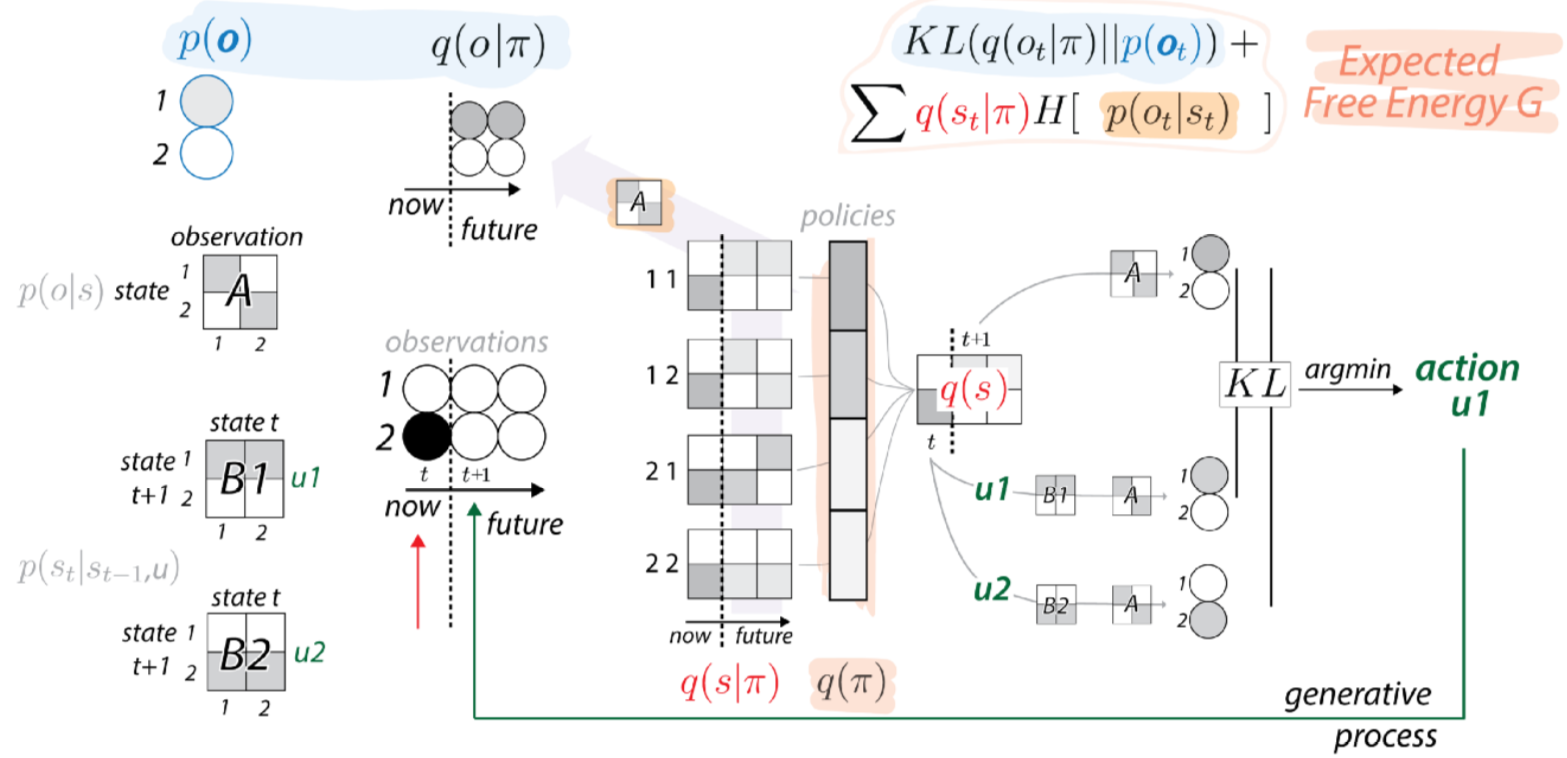
\includegraphics[width=0.7\linewidth]{14.png}}
	\end{figure}
	%\vspace{-3mm}
	
	%And to get the expected observations if we were to take a certain action, we take our belief on the hidden state at the current time step q(s\_t), multiply it by the action-specific state-transition matrix B (to get the hypothetical next state), and then by state-observation matrix A (to get the hypothetical observation). The action that minimizes the KL divergence is executed, generative process returns us the next observation at time t+1, and the process starts again. And that is it.
	
	Итак, мы никогда не моделируем действие непосредственно, а вместо этого: оцениваем скрытые состояния при каждой политике $\rightarrow$ оцениваем ожидаемую свободную энергию для каждой политики $\rightarrow$ преобразуем ее в вероятность политики $\rightarrow$ усредняем состояния для всех политик и, наконец, $\rightarrow$ действуем так, как будто мы наблюдаем то, что мы ожидаем.
	
	%So to sum up, we never actually model the action directly, but instead: estimate the hidden states under each policy -> evaluate expected free energy for each policy -> transform it to probability of policies -> average states over policies, and finally, -> act such as we observe what we expect.
	
	Формально связывание вероятности каждой политики с ожидаемой свободной энергией $G$ осуществляется следующим образом. Модель $p(o,s)$ фактически также включает в себя политику, больше похожую на $p(o,s,\pi)$. Аналогично, аппроксимация апостериорного $q$ также включает политику и выглядит как $q(s,\pi)$. Решение для оптимальной политики показано аналитически, и в дополнение к ожидаемой свободной энергии $G$, включает в себя предыдущие предпочтения [prior preferences] по политике $p(\pi)$ и свободную энергию с прошлых временных шагов (где мы фактически можем оценить точность, так как наблюдения уже известны). Однако, если мы предположим, что все политики в прошлом одинаковы -- состоят из уже выполненных действий -- аппроксимация апостериорного распределения политики $q(\pi)$ действительно зависит только от ожидаемой свободной энергии $G$ в будущем. Минимизация свободной энергии в будущем -- это <<сильно закодированный>> априор [<<hard-coded>> prior], потому что вы связываете вероятность выбора определенной политики с ее ожидаемой свободной энергией, и это дополнительное предположение, которое вы должны сделать. Это приводит к минимизации одной свободной энергии ($G$) внутри другой ($F$). Вот вариационная свободная энергия с совместным распределением, развернутым во второй строке [Here is the variational FE with the joint expanded in the second line]:
	
	%Formally, associating probability of each policy with expected FE "G" is done as follows. First, the model p(o, s) actually also includes the policy, looking more like p(o, s, pi). Similarly, the approximate posterior q also includes the policy and looks like q(s, pi). Then, the solution to the optimal policy is shown analytically, and in addition to expected FE G, include the prior preferences on the policy p(pi) and the Free Energy of the past time steps (where we actually can evaluate the Accuracy term since the observations are already known). However, if we assume that all policies in the past are the same — composed of actions already performed — approximate posterior on policies q(pi) indeed depends only on expected FE G in the future. Minimizing free energy in the future is a ‘hard-coded’ prior because you associate probability of picking a certain policy with its expected FE, and this is an extra assumption you have to make. This results in minimizing one FE (G) inside another FE (F). Here is the variational FE with the joint expanded in the second line:
	
	%\vspace{-3mm}
	\begin{figure}[h]
		\centering{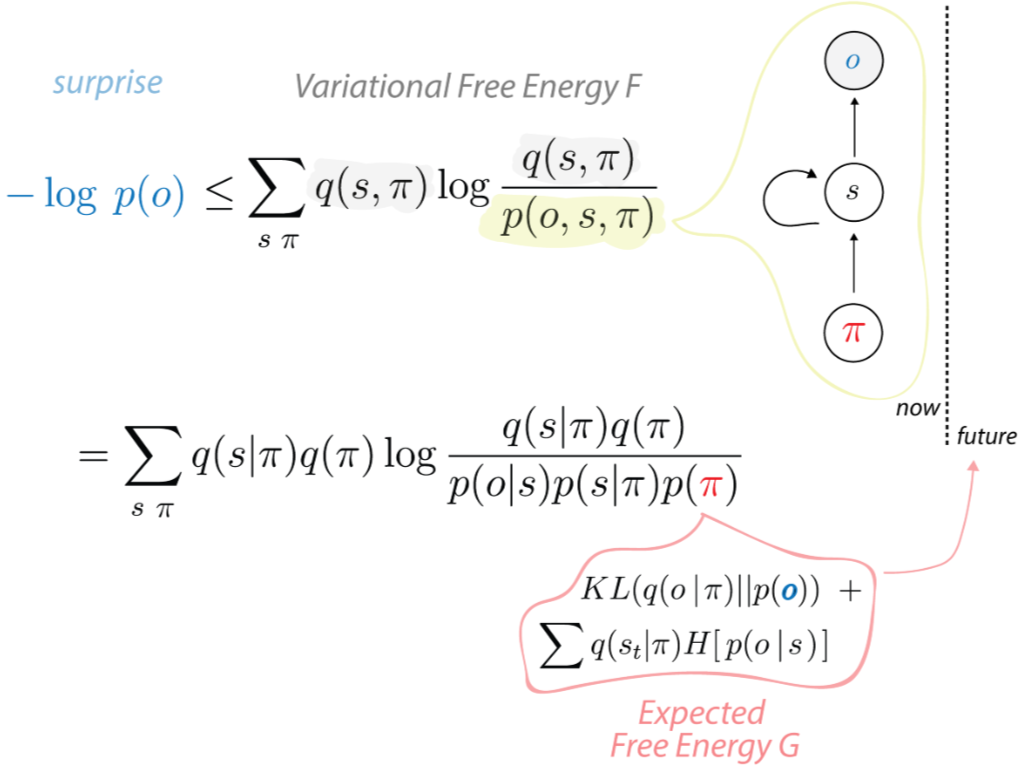
\includegraphics[width=0.6\linewidth]{15.png}}
	\end{figure}
	%\vspace{-3mm}
	
	Наконец, в дополнение к выводу, мы также изучаем параметры модели, такие, как сопоставление состояний и наблюдений (матрица $A$), переход от состояния к состоянию (матрица $В$) и точность ($\gamma$). Таким образом, минимизируя свободную энергию относительно параметров модели, мы не только делаем свободную энергию лучшим приближением неожиданности [surprise], но и минимизируем саму неожиданность.
	
	%\vspace{-3mm}
	\begin{figure}[h]
		\centering{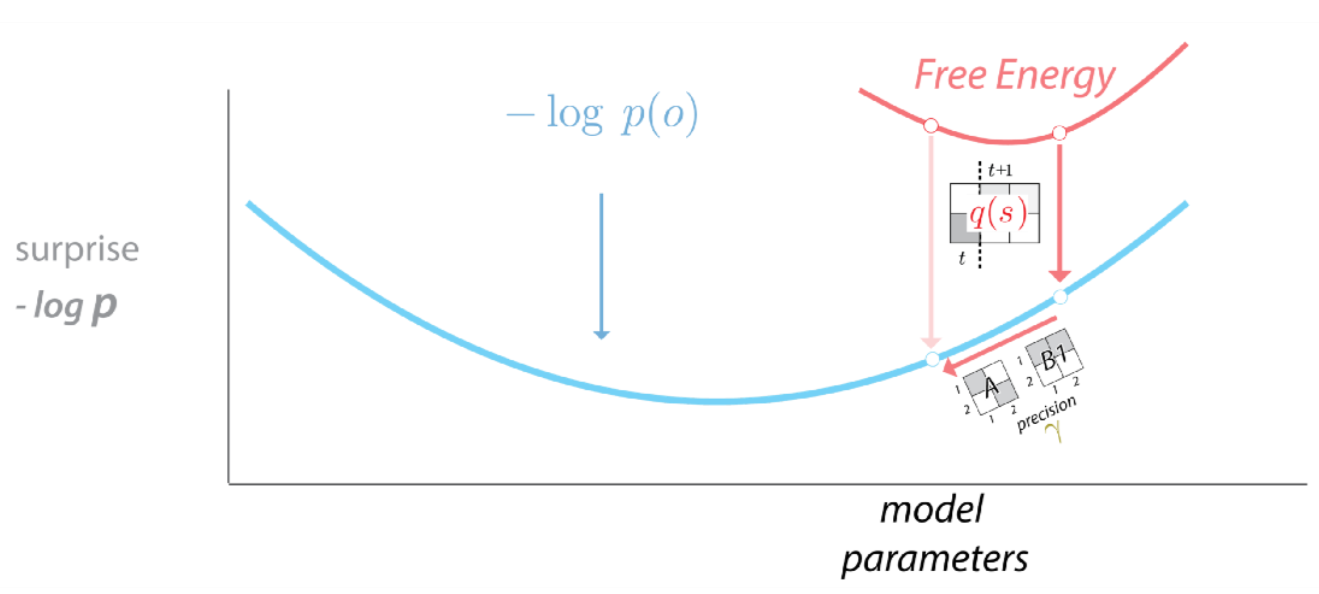
\includegraphics[width=0.7\linewidth]{16.png}}
	\end{figure}
	%\vspace{-3mm}
	
	%Finally, in addition to performing inference as discussed above, we also do learning of model parameters such as state-observation mapping (matrix ‘A’), state-to-state transition (matrix ‘B’) and precision (‘gamma’) come from. Thus, by minimizing Free Energy with respect to model parameters, we not only make Free Energy a better approximation of surprise, but also minimize surprise itself.
	
	Мы могли бы либо найти точечную оценку параметров, либо искать все распределение. В последнем случае мы включаем неопределенность параметров в нашу модель $p$, а также в аппроксимацию апостериорного $q$. Чтобы получить обоснованность модели/предельное правдоподобие/неожиданность [model evidence/marginal likelihood/surprise], мы затем суммируем не только латентные переменные, но и параметры. Таким образом, технически, поскольку мы не убрали параметры в этом посте, мы работали с вероятностью параметров $p(o|parameters, model)$ [likelihood of the parameters], но не с обоснованностью модели $p(o|model)$ [model evidence].
	
	%We could either find a point estimate (single best) parameters, or search for the entire distribution. In the later case, we include the uncertainty over parameters in our model p, as well as in posterior approximation q. In order to obtain model evidence/marginal likelihood/surprise, we would then sum out not only the latent variables but also the parameters. So technically, since we didn't marginalize parameters in this post, we worked with likelihood of the parameters p(o|parameters,model) but not model evidence p(o|model).
	
	Конечно, есть и некоторые ограничения. Например, мы предполагаем, что аппроксимации апостериорного распределения $(q_t|\pi)$ независимы в каждый момент времени, и что они раскладываются на латентные переменные и параметры. Но что еще более важно, масштабируемость этой схемы ограничена, и до сих пор моделирование включает простые ситуации с небольшими пространствами состояний и наблюдений, так что вычисления (например, определение априорных предпочтений [aprior preferences] $p(o)$, что трудно, если существует много возможных наблюдений) остаются отслеживаемыми. Однако эта схема скорее предназначена для доказательства принципа, и ее вполне достаточно, чтобы быть полезной в вычислительной психиатрии. Например, считается, что точность [precision] отражает функцию дофамина, а это означает, что неспособность определить оптимальную точность будет иметь неблагоприятные психопатологические последствия. Аналогично, в недавнем исследовании использовался активный вывод [active inference] с акцентом на мотивацию, предполагая, что люди имеют либо целенаправленные, либо однородные априорные предпочтения [prior preferences] $p(o)$. Хотя эта схема была применена к игре DOOM в OpenAI Gym, она по существу сводится к тому же самому принципу, обсуждаемому здесь, поскольку пространство состояний было дискретизировано до максимума из 10 возможных состояний.
	
	%Surely, there are some limitations too. For example, we assume that approximate posterior (q\_t|pi) is independent at each time point, and that approximate posterior factorizes between latent variables and parameters. But more importantly, the scalability of this scheme is limited, and so far, simulations involve simple situations with small state and observation spaces, so that calculations (e.g. defining the prior preferences p(o), which is hard if there are many possible observations) remain tractable. However, the scheme is rather intended as a proof of principle, and is sufficient to be useful in computational psychiatry. For example, precision is believed to reflect the function of dopamine, meaning that inability to infer the optimal precision would have adverse psychopathological implications. Similarly, a recent study used active inference with a focus on motivation, by assuming that people have either goal-oriented or uniform prior preferences p(o). While the scheme was applied to the game of DOOM in OpenAI Gym, it essentially boils down to the same principle discussed here, since the state space has been discretized to a maximum of 10 possible states.

\end{document}]